% PFC: PhotoPlace
% (c) Jose Riguera Lopez 2013

% Opciones:
%       a4paper -> indica el tamaño del papel, en este caso A4.
%       11pt    -> tamaño de la fuente 11 puntos.
%       twoside -> doble cara.
%       oneside -> una cara del folio.
%
\documentclass[a4paper,11pt,twoside]{book}
%% Estilo PFC UDC
\usepackage{pfc}
%% Macros
\newcommand{\curso}{Enxeñaría en Informática}
\newcommand{\proyecto}{Proxecto Fin de Carreira}
\newcommand{\universidad}{Universidade de A Coruña}
\newcommand{\centro}{Facultade de Informática}
\newcommand{\unicentro}{\centro da \universidad}
\newcommand{\proyectotipo}{Proxecto clásico de enxeñaría}
\newcommand{\titulo}{Servicio en línea para la publicación de grabaciones de radio y podcasts}
\newcommand{\titulogalego}{Servizo en liña para a publicación de gravacións de radio e podcasts}
\newcommand{\tituloenglish}{Online service for publishing radio broadcasting recordings and podcasts}
\newcommand{\corto}{Servizo de publicación de gravacións de radio}
\newcommand{\autor}{Fernando Liñares Varela}
\newcommand{\director}{José María Casanova Crespo}
\newcommand{\tutor}{}
\newcommand{\departamento}{Departamento de Computación}
\newcommand{\software}{PhotoPlace}
\newcommand{\palabras}{Radio, Podcast, Web, Django, Postgres, Python, Javascript, jQuery, CSS Grid. }

\renewcommand{\spanishtablename}{Táboa}

\title{\titulo}
\author{\autor}
\date{\today}

\hypersetup{
%   bookmarks=true,         % barra de marcadores
    unicode=false,          % caracteres non-Latin en marcadores de Acrobat
    pdftoolbar=true,        % mostrar barra de herramientas de Acrobat
    pdfmenubar=true,        % mostrar menú de Acrobat
    pdffitwindow=false,     % ajustar ventana al ancho de página
    pdfstartview={FitH},    % ajustar documento al ancho de página
    pdftitle={\corto},      % título
    pdfauthor={\autor},     % autor
    pdfsubject={\titulo},   % tema del documento
    pdfcreator={LaTex},     % generador del documento
    pdfproducer={\autor},   % productor del documento
    pdfkeywords={\palabras},% lista de palabras clave
    pdfnewwindow=true,      % enlaces en una nueva ventana
    colorlinks=true,        % false: enlaces en caja; true: enlaces coloreados
    linkcolor=black,        % color de enlaces internos
    citecolor=green,        % color de enlaces a bibliografía
    filecolor=magenta,      % color de enlaces a ficheros
    urlcolor=blue           % color de enlaces externos
}

%\loadglsentries{pfc.glossary}
\makeglossaries

\begin{document}
  \graphicspath{{./images/}}
  % pageblank genera una pagina en blanco, para imprimir en formato libro
  %
% Portada.
%
\begin{titlepage}
	\begin{center}
		% Logotipo de la universidad.
		
\includegraphics[width=6cm]{./eps/logo_udc.eps}
		\vspace{2cm}

		% Nombre de la facultad, de la universidad y del departamento.
		{\Large{\textbf{\centro}}}
		\\
		{\it \large{\textbf{\departamento}}}
		\vspace{1cm}

		{\large {\sc \proyecto}\\{\curso}}
		\vspace{1cm}

		% Título
		\textbf{\Large \titulogalego}
		\vspace{6cm}
	\end{center}

	\begin{flushright}
		\begin{tabular}{ll}
			\large{\textbf{Alumno:}}	&
			\large{\autor} \\

			\large{\textbf{Director:}}	&
			\large{\director} \\

			\large{\textbf{Tutor:}}		&
			\large{\tutor} \\

			% Fecha.
			\large{\textbf{Fecha:}}		&
			\large{\today} \\
		\end{tabular}
	\end{flushright}
\end{titlepage}

  \pageblank
  %
% Certificado
%
\thispagestyle{plain}
\begin{center}
	\begin{minipage}[t][6cm][l]{.8\textwidth}
		\begin{center}
			% Director del proyecto
			D. {\sc \director}

			% Profesores
			Profesor, \centro

			% Departamento al que pertenece el director y en el que se realiza el proyecto.
			\departamento
			
			\universidad
		\end{center}
	\end{minipage}
\end{center}

CERTIFICA:

Que la memoria titulada {\it ``\titulo''} ha sido realizada por {\sc \autor}
de acuerdo a la descripción inicialmente propuesta, bajo mi dirección y
constituye su {\proyecto} de {\curso}.
Por la presente, autorizo su presentación para que el Proyecto sea defendido
en esta convocatoria.

\vspace{3cm}

En A Coruña, a \today

% Espacio para que pueda firmar el certificado que debe acompañar al proyecto.
\vspace{3cm}
\begin{center}
	\begin{minipage}[t][4cm][l]{.5\textwidth}
	D. {\sc \director}
	\\
	Director del proyecto
	\end{minipage}
\end{center}

  \pageblank
  %
% Nota
%
\thispagestyle{plain}
\section*{}


\begin{tabular}{p{2cm}p{11cm}}
	\large{Título} & \\
	& \textbf{\large{\titulogalego}} \\
	\\
	& \textbf{\large{\titulo}} \\
	\\
	& \textbf{\large{\tituloenglish}} \\
	\\
	\large{\textbf{Clase:}} & \large{\proyectotipo} \\
	\\
	\large{\textbf{Autor:}} & \large{\autor} \\
	\large{\textbf{Tutor:}} & \large{\tutor} \\
	\large{\textbf{Director:}} & \large{\director} \\
	\large{\textbf{Data:}} & \large{\today} \\
	\\
	\large{\textbf{Tribunal}} & \\
	& \vspace{3cm} \\
	\\
	\large{\textbf{Data de defensa:}} & \\
	\\
	\large{\textbf{Calificación:}} & \\
	\\
\end{tabular}

  \pageblank
  \thispagestyle{plain}
\section*{Resumo}


   

  \pageblank
  \thispagestyle{plain}
\section*{Lista de Palabras Clave}

{\setlength{\parindent}{0cm}\ttfamily
\palabras
}



  \pageblank
  %
% Dedicatoria
%
\thispagestyle{plain}

\begin{flushright}
	{\it A todo el mundo.}
\end{flushright}

  \pageblank
  %
% Agradecimientos
%
\chapter*{Agradecimientos}
\vspace*{2cm}

A los profesores {\director} por sus consejos durante el desarrollo del proyecto.  POR HACER\\



  \pageblank
  
  % FRONTMATTER: TOC, LOF, LOT
  \frontmatter
  \dominitoc[n]     % removes the title "contents"
  \nomtcrule        % removes rules = horizontal lines
  \tableofcontents
  %\addcontentsline{toc}{chapter}{Contents}
  \listoffigures
  %\addcontentsline{toc}{chapter}{List of Figures}
  %\listoftables
  %\addcontentsline{toc}{chapter}{List of Tables}

  % MAINMATTER: content
  \mainmatter
  \chapter[Introducción]{
  \label{chp:introduccion}
  Introducción
}
\minitoc
\newpage

El proceso de desarrollo del software comienza con un análisis del entorno y
del dominio de la aplicación. En un contexto amplio, se entiende por dominio
como ``una esfera de actividad o interés'', también denominado campo. Es decir,
el área de aplicación donde el software fue creado.

En el presente capítulo se describe el entorno y el dominio de la aplicación, y la
evolución de los servicios de geolocalización en los últimos años. A su vez,
también se exponen los objetivos de este proyecto, dando una visión
de su estructura y las partes que la forman.


\section{Dominio de Aplicación}

La evolución de los \glspl{SIG} ha sido imparable en la ultima década. Motivado 
-sin duda- por el interés de gigantes tecnológicos como Google, Apple y Microsoft, 
ha provocado que se hayan popularizado y extendido tecnologías que  antes sólo 
estaban al alcance de profesionales y científicos.


  \include{estado_da_arte}
  \chapter[Tecnoloxías Utilizadas]{
  \label{chp:tecnologia}
  Tecnoloxía
}
\minitoc
\newpage

Este capítulo contempla a base tecnolóxica utilizada na última versión do proxecto até a data
de entrega desta memoria. Os conceptos listados nesta sección están suxeitos a posibles cambios
por mor dos futuros traballos de actualización e despregue nun entorno de produción que se pretenden
efectuar. 

Á hora de elixir o uso destas ferramentas valorouse a súa natureza open source xa que se pretende que o
resultado dispoña dunha licencia de software libre compatible coa definición da Free Software
Foundation. 

Tamén se valoraron, dado que nos capítulos anteriores insistiuse na importancia dos dispositivos móviles
no consumo da radio a través de Internet, as posibilidades de ditas ferramentas de ofrecer un bo resultado
en distintos dispositivos e distintas plataformas software. 


\section{Linguaxes}

\subsection{Python}
\label{python}
Python é unha linguaxe de propósito xeral de alto nivel. Trátase dunha linguaxe interpretada polo que é necesario 
ter un intérprete para executar o código. Ao ser o intérprete unha capa intermedia de software entre o programa
e o sistema, Python é unha linguaxe fácilmente portable entre dispositivos de distinta natureza.

A súa sintaxe baseada na indentación está pensada para favorecer a comprensión entre distintos desenvolvedores e 
facilitar o mantemento do código. 

O seu sistema de tipado implícito e a súa riqueza de bibliotecas para executar comandos de consola de xeito programático
fan que sexa moitas veces descrito coma \say{unha linguaxe de scripting orientada a obxectos}\cite{python1}, o cal serve coma 
mostra da súa flexibilidade, un dos motivos polo que foi elixida para este proxecto.

\subsubsection{Anaconda}

Anaconda é unha distribución de Python, libre e de código aberto (licenza BSD), utilizada normalmente para análise estatística e machine learning. Inclúe, ademáis dunha completa instalación do intérprete de Python, un rico conxunto de librarías de uso común e o xestor de paquetes conda, sendo esas dúas últimas melloras o motivo primordial polo que foi a elección para este proxecto. Conda utiliza os paquetes da comunidade de Conda Forge \cite{anaconda1}

Anaconda é responsabilidade de Anaconda Incorporated, antigo Continuum Analytics.

A versión utilizada foi a Anaconda 4.4.0 de 64 bits para Python 3, a máis nova no momento de comezar o traballo. Inclúe o intérprete para Python versión 3.6.1.


\subsection{HTML}

HTML (acrónimo de HyperText Marckup Language) é a linguaxe estándar para a creación da estrutura das páxinas web. Os 
elementos presentes na web declaranse mediante bloques representados por etiquetas(tags), de ahí que reciba o nome de
\say{marckup language} (linguaxe de marcado). Estas etiquetas son interpretadas polos navegadores para renderizar o 
contido da páxina\cite{html1}. Ao ser un estándar tan lonxevo, consolidado e popular, non se consideraron alternativas 
para este proxecto.

Dado á natureza multimedia da web realizada, utilizouse HTML5. Esta quinta revisión do estándar inclúe novas etiquetas 
para o tratamento das imaxes e dos contidos de audio e vídeo sen necesidade de utilizar outras tecnoloxías complementarias, 
simplificando así o desenvolvemento e o mantemento posterior do portal. Desde decembro do pasado ano 2017, a versión 5.2 é a última estable recomendada polo World Wide Web Consortium(W3C)\cite{html_w3c}.


\subsection{CSS}

CSS (Acrónimo de Cascading Style Sheets) ou \say{Follas de estilo} é unha linguaxe empregada para definir a estética dos elementos definidos anteriormente no código HTML: A súa cor, fonte, posición... Ao separar o estilo da estrutura, favorécese a reutilización de código xa que un mesmo ficheiro de CSS pode ser utilizado en diversas páxinas ao mesmo tempo. CSS permite tamén adaptar o contido das páxinas a dispositivos de distinto tamaño\cite{css_w3c}.

\subsubsection{CSS Grid}

O módulo de \say{Grid} úsase para definir un deseño de interface gráfica consistente nunha cuadrícula de dúas dimensións en CSS. Nun modelo deste tipo, declárase un conxunto de elementos no HTML coma pertencentes a un \say{grid container}(contedor da grella ou da cuadrícula) e, á súa vez, zonas fillas que se posicionarán dentro dese contedor dependendo das características coas que este último fose definido na folla de estilos.

Unha cela nun contedor pode, á súa vez, consistir noutro contedor, permitindo así deseños asimétricos. O tamaño das celas pode ser fixo, relativo á páxina ou automático dependendo do contido da cela. Por todo o dito, este módulo proporciona un nivel de flexibilidade superior ao que poderíamos obter utilizando outras alternativas populares coma CSS Flexbox. 

O nivel primeiro de CSS Grid non acadou aínda, na data de entrega desta memoria, o status de \say{recomendación} da  World Wide Web Consortium(W3C)\cite{css_grid_w3c}, porén, xa é soportado polas últimas versións dos navegadores máis populares\cite{css_grid_w3c2} polo que non se considerou un risco utilizalo neste proxecto.

\subsection{JavaScript}

JavaScript é unha linguaxe de scripting interpretada e de alto nivel. Utilízase principalmente (e tamén neste proxecto) coma unha ferramenta para mellorar a interactividade da interface web ao permitir executar código orientado a eventos no lado do cliente, aforrando recargas da páxina e incluso accesos innecesarios á base de datos xa que permite o uso do disco local mediante cookies. 

A pesares do seu nome, non garda relación algunha coa linguxe Java e serven a propósitos claramente distintos. O núcleo desta linguaxe está regulado polo estándar ECMAScript\textregistered, na súa 8\textsuperscript{a} versión\cite{ecma} no momento de entregar esta memoria. 

Como se comentou no apartado \ref{python}, que sexa interpretada implica a necesidade dun intérprete para executar o código. Ese intérprete, comunmente chamado JavaScript Engine preséntase embebido nos navegadores web. Non obstante, non éxiste unha única implementación senón que distintos navegadores presentan distintas versións. Para o desenvolvemento deste proxecto utilizáronse os navegadores Mozilla Firefox 57.0.1 e Google Chrome 66.0, cuxos motores de JavaScript son SpiderMonkey e V8 respectivamente\cite{javascript1}, ambos os dous libres e de código aberto.

Pese a que o seu uso nos navegadores continúa a ser a principal razón de ser desta linguaxe, tamén se utiliza a día de hoxe noutro tipo de produtos coma Node.js(para correr JavaScript no lado do servidor) ou Apache Couch DB (Para o manexo de bases de datos na nube)\cite{javascript2} 


\subsection{SQL}

SQL é a linguaxe utilizada para a manipulación dos datos dentro do eido das bases de datos relacionais. Nace coma un refinamento ou \say{secuela} (SQL é unha simplificación da verba inglesa \say{sequel}) da linguaxe SQUARE, que á súa vez consistía nunha simplificación da linguaxe DSI/Alpha proposta polo mesmo Edgar F. Codd no momento de presentar o modelo relacional de Bases de Datos. O primeiro estándar foi publicado no ano 1986 pola American National Standards Institute (ANSI)\cite{sql1}. Permite definir a estruturación dos datos, insertalos, eliminalos, editalos e, por suposto, consultalos.

Neste proxecto, o seu uso explícito correspóndeuse só coas primeiras fases do traballo debido á utilización do framework Django coma se detalla no apartado \ref{django}. É necesario especificar tamén que, pese á existencia dun estándar, existen distintas versións desta linguaxe que a fan \say{non completamente portable} entre distintos sistemas de xestión de bases de datos\cite{sql2}. Neste proxecto utilizouse a variante correspondente a PostgreSQL.


\subsection{XML}

XML é o acrónimo de \say{eXtensible Markup Language} (Linguaxe de marcado extensible). Consiste nunha serie de normas que dividen un documento en distintas partes, asignándolle unha identidade a cada unha delas. A diferencia doutras linguaxes de marcado coma o HTML, non existe un conxunto de etiquetas válido. No XML queda á responsabilidade do autor do documento establecer as etiquetas necesarias dependendo do entorno no que ese documento vaia ser utilizado. Por suposto, existen unha serie de normas estruturais para que o etiquetado se poida considerar coma válido, pero desde o punto semántico, a natureza destas etiquetas é moi flexible. Isto fai que moitas veces se denomine o XML coma unha Meta-Linguaxe, é dicir, unha linguaxe para definir linguaxes\cite{xml1}.

A función de XML é definir a semantica e a estrutura dun documento, pero nunca o estilo. Ao igual que HTML, pódese asociar unha folla de estilos CSS.

Neste proxecto, XML é utilizado na súa modalidade RSS do xeito detallado no apartado \ref{rss}.

\subsubsection{RSS}
\label{rss}

RSS é un tipo de formato XML utilizado para a \say{sindicación} web, isto é, a emisión de contidos actualizados dunha páxina web a un número indefinido de subscriptores. Utilízase para evitar a procura manual de novos contidos naquelas páxinas nas que a actualización é frecuente: Páxinas de novas, blogs, podcasts... 

O seu funcionamento consiste nun ficheiro RSS (comunmente chamado \say{feed}) accessible desde a web polos programas clientes de rss que posúan os subscriptores. Ese feed mostra información resumida do contido publicado no sitio web ao que fai referencia. Cada vez que o contido se actualice, o feed actualizarase tamén e ese cambio será detectado polo cliente rss de xeito automático.
 
O nome procede do acrónimo de \say{Really Simple Syndication}(Sindicación Realmente Sinxela) e o estándar é mantido polo \say{RSS Advisory Board}. Na data de entrega desta memoria e desde o ano 2009, a última revisión é a 2.0.11 \cite{rss}

Neste proxecto, o interese céntrase na actualización dos podcasts. Existen alternativas a este formato de sindicación mais, dado o seu uso xeralizado entre os usuarios potenciais da aplicación web a desenvolver, non foron consideradas.


\section{Django Framework}
\label{django}
O proxecto Django nace no ano 2005 coma un conxunto de ferramentas Python para o desenvolmento web publicadas
baixo licencia BSD. A motivación dos seus creadores, Simon Wilson e Adrian Holovaty, naquel tempo programadores
nun medio periodístico, era a homoxeneización e a reutilización de código. Isto daba resposta á necesidade de reducir
o alto custo que supón manter código ad-hoc para cada novo artigo ou función, especialmente nunha páxina que
requira unha constante actualización de contidos coma a dun diario online. É por iso que se adoita utilizar o 
termo \say{newsroom schedule} cando se fala da rapidez de desenvolvemento que permite o framework\cite{django1}.  

Django ofrece un conxunto de bibliotecas que dan soporte ás mecánicas máis comúns do desenvolvemento
web:

\begin{itemize}
	
	\item Persistencia: Django permite crear a estrutura da base de datos sen necesidade de escribir SQL. Isto 
	conséguese mediante a superclase Model da librería \say{db} de Django. Ao declarar unha clase de Python coma
	extensión de \say{Model}, a biblioteca ocúpase automáticamente de manter a coherencia entre as súas instancias en 
	memoria e as táboas da base de datos. 
	
	\item Peticións web: A lectura e a interpretación destas peticións son levadas a cabo polo conxunto de bibliotecas
	de HTTP do framework, encapsulando as peticións e as respostas en obxectos para formar un estándar sinxelo e garantir
	a correcta formación das mesmas.
	
	\item Enrutamento e Validación: O framework ofrece un estándar para asignar as distintas vistas definidas no código
	ás URL's desexadas. Os posibles formularios presentes nesas vistas poden ser abstraídos en obxectos de Python 
	simplificando a validación dos datos introducidos polos usuarios. A utilización destes sistemas é non obstante, 
	opcional, puidendo o programador optar por utilizar sinxelos formularios HTML no caso de que isto axilizase 
	o desenvolvemento.
	
	\item Sistema para embeber datos dinámicos no HTML: O chamado \say{template system} de Django marca uns procedementos
	sinxelos para acceder aos datos xenerados no código. Tamén ofrece ferramentas para implementar certa lóxica
	presentacional.
	
	\item Interface de administración nativa: Por defecto, este framework dispón dun panel de administración de acceso
	reservado aos superusuarios que evita os accesos directos á base de datos no caso de que un administrador necesite
	facer cambios manuais nos datos.
	
	\item Soporte por defecto para a autenticación e autorización: Django permite ao desenvolvedor invocar a clase 
	nativa Usuario e efectuar con ela accións de rexistro, autenticación e concesión/revocación de permisos sen máis
	programación. Se ben, como se explica máis adiante, neste proxecto extendeuse esa clase Usuario e creouse unha
	xerarquía de permisos propia.

\end{itemize}   


Para este proxecto utilizouse concretamente Django 1.11, a versión estable máis avanzada no tempo en que se comezou o 
traballo. Django sufriu unha actualización importante desde entón que rematou coa publicación de Django 2.0 en Decembro do pasado ano 2017. Estas dúas versións non son totalmente compatibles de modo que unha actualización implicaría cambios no 
código. Tendo en conta que a Django Software Foundation, responsable do mantemento do framework, non prevee retirar o soporte á versión utilizada nun futuro próximo e que a versión de Python utilizada é soportada tamén por Django 2\cite{django2}, considerouse aceptable o grao de actualidade da tecnoloxía utilizada.    

Ademáis do mencionado anteriormente, confiouse en Django para este proxecto pola súa madurez e pola súa popularidade, sendo  utilizado en sitios coma Instagram, Disqus, Pinterest ou Open Knowledge Foundation.


  \chapter[Metodoloxía]{
  \label{chp:metodoloxia}
  Metodoloxía
}
\minitoc
\newpage

A metodoloxía de traballo baseouse nos principios das \textbf{metodoloxías áxiles} aplicando, concretamente, aquelas prácticas e técnicas de \textbf{\say{Extreme Programming}} (XP) adaptables ao traballo individual. Destacarase, pola súa especificidade, o uso da técnica de \say{Test Driven Development} (TDD) nalgunhas partes do desenvolvemento.

\section{Principios das metodoloxías áxiles}

Considéranse áxiles aquelas metodoloxías motivadas por unha serie de valores e que respectan unha serie principios, ambos recollidos no \say{manifesto áxil} do ano 2001 \cite{axiles}. Eses valores son:

\begin{itemize}
	\item \textbf{Os individuos e súa interacción} valórase máis que as ferramentas e os procesos.
	\item \textbf{O correcto funcionamento do software} valórase máis que a documentación extensiva.
	\item \textbf{A colaboración co cliente} valórase máis que a negociación contractual.
	\item \textbf{A resposta ante o cambio} valórase máis que o seguimento dun plan.
\end{itemize}

Que se traducen nos chamados \textbf{\say{Doce principios do Software Áxil}}:

\begin{enumerate}
\item A nosa maior prioridade é satisfacer ao cliente
mediante a entrega temperá e continua de software
con valor.

\item Aceptamos que os requirimentos cambien, incluso en etapas 
tardías do desenvolvemento. Os procesos Áxiles aproveitan
o cambio para proporcionar vantaxe competitiva ao 
cliente.

\item Entregamos software funcional frecuentemente, entre dúas
semanas e dous meses, con preferencia ao período de 
tempo máis corto posible.

\item Os responsables de negocio e os desenvolvedores
traballamos xuntos de forma cotiá durante todo
o proxecto.

\item Os proxectos desenvólvense en torno a individuos 
motivados. Hai que darlles o entorno e o apoio que 
necesitan, e confiarlles a execución do traballo. 

\item O método máis eficiente e efectivo de comunicar 
información ao equipo de desenvolvemento e entre os seus 
membros é a conversación cara a cara.

\item O software funcionando é a medida principal de 
progreso.

\item Os procesos Áxiles promoven o desenvolvemento 
sostible. Los promotores, desenvolvedores e usuarios
debemos ser capaces de manter un ritmo constante 
de forma indefinida.

\item A atención continua á excelencia técnica e ao 
bo deseño mellora a Axilidade.

\item A simplicidade, a arte de maximizar a cantidade de
traballo non realizado, é esencial.

\item As mellores arquitecturas, requirimentos e deseños
emerxen de equipos auto-organizados.

\item A intervalos regulares o equipo reflexiona sobre
como ser máis efectivo para a continuación axustar e
perfeccionar o seu comportamento en consecuencia.
\end{enumerate}


\section{Extreme Programming}

Extreme Programming (XP), ou Programación Extrema, é un estilo de desenvolvemento de software que promove unha serie de valores de cara ao traballo en equipo e unha serie de técnicas que supoñen unha simplificación e unha alternativa flexible en contraposición a outras metodoloxías máis tradicionais coma, por exemplo, o \say{desenvolvemento en fervenza}.

Eses valores enuméranse coma\cite{xp}: 

\begin{itemize}
	\item \textbf{Comunicación:} Tanto entre programadores coma co cliente.
	\item \textbf{Simplicidade:} Que o código sexa lexible e a documentación concisa.
	\item \textbf{Retroalimentación:} Realizar iteracións curtas para obter opinións rápidas sobre os progresos.
	\item \textbf{Coraxe:} Aceptar que a aparición de novos requirimentos é natural e poden redefinir o deseño.
	\item \textbf{Respecto:} Estrutura horizontal do equipo de desenvolvemento.
\end{itemize}


A posta en práctica dos anteriores valores lévanos a unha metodoloxía de traballo baseada no contacto continuo co cliente para poder obter correccións e ideas novas (retroalimentación). Isto acádase mediante ciclos curtos de desenvolvemento, ao final dos cales volveremos reunirnos co usuario obxectivo e o ciclo volve a comezar. 

Referímonos a estes ciclos coma \textbf{iteracións} e a esas \say{ideas novas} coma \textbf{historias de usuario}. Poden ser tomadas coma unha planificación do traballo a curto prazo a entender non coma unha improvisación, senón coma unha peza dun plan global suxeito á evolución do proxecto.

Debido á aceptación de que os sucesivos cambios no deseño son inevitables (coraxe) e que a refactorización de código é algo necesario para asegurar a súa cualidade (simplicidade), faise necesaria a automatización de probas e a utilización dun control de versións.

A metodoloxía XP ten unha serie de características aplicables ao traballo en equipo que non se levaron a cabo neste proxecto: A programación por parellas, a revisión de código entre desenvolvedores ou a división do traballo en función da especialización do persoal (Testers, deseñadores de interacción, directores do proxecto, programadores...)

\subsubsection{Aporte da metodoloxía ao proxecto}

Ao ser este un Proxecto de Final de Carreira, as reunións co cliente substituíronse por \textbf{reunións co director do proxecto de periodicidade quincenal}. Nelas, revisábanse os progreso e xurdían novas historias de usuario (ou se actualizaban as vellas). Grazas a este modo de traballo conseguíronse identificar varios \textbf{requirimentos non valorados a priori} coma, por exemplo, a necesidade de establecer roles de usuario. 

Para afondar individualmente en cada iteración, ver o capítulo \ref{chp:plan} sobre a planificación.


\section{Test Driven Development}

Test Driven Development (TDD) é unha técnica utilizada nas metodoloxías áxiles de desenvolvemento que segue a filosofía \textbf{probar primeiro}. Esta baséase na conversión dos requirimentos en probas antes da propia existencia de código que as avale. Isto obriga ao desenvolvedor a pensar nos requirimentos con detemento, identificar de antemán os posibles fallos e aumentar o alcance da validación de datos. Unha vez o test está definido, pasarase a implementación da funcionalidade posta a proba. De pasar a proba, repítese co seguinte requirimento. Este ciclo pode verse no esquema da figura \ref{fig:tdd}.

\begin{figure}[h]
	\centering
	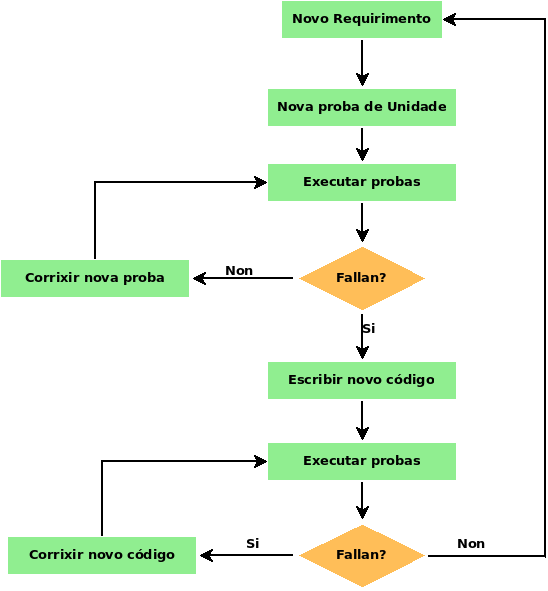
\includegraphics[scale=0.55,keepaspectratio=true]{./images/TDD.png}
	\caption{Diagrama do ciclo de desenvolvemento coa metodoloxía TDD.}
	\label{fig:tdd}
\end{figure}

Existen distintas estratexias á hora de seguir o citado ciclo \cite{tdd} que se poden utilizar en función das características do requirimento:

\begin{itemize}
	\item \textbf{Fake it ('til you make it):} Ou \say{falséao (ata que o fagas)}. Baséase en escribir primeiro un método falso que devolva un valor constante que satisfaga o test. A partir de aí, ilo modificando aos poucos sempre vixiando que o test sexa positivo até que o método estea completo. Esta práctica é moi complexa de utilizar se os métodos son grandes, polo que pode ser unha boa forma de forzar a división, algo desexable para a cualidade do código.
	
	\item \textbf{Triangulación:} Consiste en facer as mesmas comprobación 2 ou máis veces con parámetros distintos dos que esperemos unha saída distinta coa fin de abstraer a función a implementar a raíz dos resultados esperados. Esta implementación é útil para evitar os parámetros superfluos que poidan aparecer nas funcións complexas.
	
	\item \textbf{Implementación Obvia:} Para as funcionalidades sinxelas, non paga a pena utilizar estratexias de abstracción. Podemos simplemente implementar o método e agardar a que o test non falle. Queda a discreción do desenvolvedor definir que funcións son sinxelas e complexas.
	
	\item \textbf{Un a Moitos:} No caso daqueles métodos que actúan sobre unha pluralidade de obxectos, esta estratexia avoga por dividir o requirimento en dous: Habería que validar primeiro o un método que actuaría sobre unicamente un obxecto e, a continuación, validar que se execute sobre dita colección.  

\end{itemize}


Neste proxecto, seguiuse maioritariamente a terceira estratexia da anterior lista por resultar máis intuitiva para o traballo a realizar.

\subsubsection{Aporte da técnica ao proxecto}

Considerouse a utilización de TDD durante a \textbf{implementación do modelo de datos} (ver primeiras iteracións no capítulo \ref{chp:plan}), ao predicirse que sería un código moi sensible aos cambios podería dar pé a regresións. Tamén axudou ao análise de requirimentos ao forzarnos a pensar nos resultados posibles de cada método de antemán.

O uso de TDD forzou a temperá implementación de probas automatizadas, que se poden ver detalladas no capítulo \ref{chp:test} sobre as probas do sistema.



  \chapter[Análise]{
  \label{chp:analise}
  Análise
}
\minitoc
\newpage

Neste capítulo descríbese o funcionamento ideal da aplicación. Exporanse tamén os requirimentos funcionais e non funcionais identificados ao abordar os obxectivos do proxecto. 

\section{Descrición do funcionamento}

O sistema consiste nunha páxina web con apartados adicados, por un lado, ao que chamamos actividades de consumo, e por outro ás actividades de produción.

\subsection{Actividades de consumo de contidos}

Son aquelas \textbf{levadas a cabo polos ouvintes} das emisoras e os programas presentes no sistema. Un usuario, no seu papel de \say{consumidor}, pode, mediante a interface web, acceder ao catálogo de programas, xa sexa mediante as ferramentas de busca proporcionadas ou a través das recomendacións que a propia páxina amosa en portada.

Dentro da páxina correspondente a unha emisora, o usuario atopará un reprodutor HTML5 desde o que \textbf{escoitar a súa emisión en directo} mediante streaming. O usuario terá opción de \textbf{facerse \say{seguidor}} da emisora para acceder a ela de xeito máis rápido desde a páxina principal.

Tamén obterá acceso á lista de programas emitidos por dita emisora co seu horario de emisión. Na páxina de cada programa verá a lista completa de episodios dispoñibles e terá a opción de \textbf{subscribirse} para poder acceder de xeito máis rápido aos novos episodios publicados.

Na páxina propia de episodio atopará outro reprodutor HTML5 que lle posibilitará ou ben a escoita por streaming ou ben a \textbf{descarga directa do ficheiro de audio} correspondente. Poderá votar o programa a favor ou en contra (isto repercutirá na popularidade do programa, concepto explicado máis adiante) e deixar un comentario no caso de que esta opción esté habilitada polos administradores do programa.


\subsection{Actividades de produción de contidos}

Son aquelas levadas a cabo polos \textbf{propietarios e administradores} dos programas e emisoras. Un usuario, no seu papel de produtor, poderá engadir ao sistema unha \textbf{nova emisora} cubrindo o formulario habilitado a tal efecto na interface web no que deberá introducir manualmente os datos.

Poderá tamén \textbf{engadir un programa}. Para isto, o usuario só necesitará proporcionarlle ao sistema un enlace ao ficheiro de RSS do podcast que queira engadir e o sistema encargarase de extraer a información tanto dos programas coma dos episodios correspondentes. Este programa e os seus episodios manteranse actualizados xa que o propio backend do sistema comprobará periodicamente se houbo algún cambio no RSS e actualizará a base de datos de xeito acorde.  

Un usuario que posúa un programa ou emisora pode invitar a outro usuario a \textbf{colaborar na xestión} desta ou deste.


\section{Requirimentos funcionais}

Son aqueles que describen as \textbf{accións que o sistema debe efectuar}, isto é: a colección de capacidades e características que o software pon a disposición do usuario. Presentaranse estes en forma de \textbf{historias de usuario} (ver capítulo \ref{chp:metodoloxia} sobre a metodoloxía). 

Se ben é certo que houbo \textbf{encontros con membros de colectivos do terceiro sector} coma a URCM (Unión de radios libres e comunitarias de Madrid) e Cuac FM (A radio comunitaria da Coruña), parte delas están extraídas da \textbf{experiencia propia} coma colaborador nestes medios e coma moderador de comunidades en liña.


\begin{itemize}
	\item Ter un punto de encontro onde ver os programas que están a emitir as emisoras federadas na ReMC (Red de Medios Comunitarios)
	\item Que unha emisora poda acceder aos ficheiros de audio das demais.
	\item Que os \say{autores} dun programa poidan saber en que emisoras está a ser emitido e a que hora.
	\item Que os programas se poidan dar de alta e de baixa.
	\item Poder visualizar información das emisoras e dos programas: Nome, información de emisión, datos de contacto...
	\item Poder subscribirse aos programas.
	\item Poder compartir contido entre usuarios.
	\item Que os ficheiros de audio se asocien de xeito automático a cada emisora.
	\item Que non sexa necesario engadir manualmente os novos ficheiros.
	\item Que os usuarios podan colaborar na xestión das emisoras.
	\item Agrupar os programas por categorías.
\end{itemize}

Eses \say{ficheiros de audio} nos que se pensaba nunha primeira aproximación foron o que finalmente derivou no concepto de \say{episodios de programa} que se explicará máis a fondo no capítulo \ref{chp:disenho} sobre o deseño.

Gran parte destas historias veñen dos usuarios que producen o contido. A medida que avanzaba o deseño e os primeiros pasos da implementación, fóronse perfilando novas historias de usuario pensando máis nos ouvintes:

\begin{itemize}
	\item Que os ouvintes poidan manifestar a súa opinión sobre os programas mediante votos e comentarios.
	\item Que os ouvintes poidan manter unha lista de programas e emisoras favoritas.
	\item Ter ferramentas de procura de contidos.
	\item Recibir recomendacións.  
\end{itemize}  

E tamén outros requirimentos propios da xestión dos contidos.

\begin{itemize}
	\item Crear diferentes roles de administración.
	\item Que o administrador dun programa poida restrinxir a emisión do seu contido.
	\item Que o administrador dun programa poida moderar os comentarios no seu contido.
\end{itemize}  

\section{Requirimentos non funcionais}

Son aqueles que \textbf{especifican as propiedades do sistema} no referente á manexabilidade, seguridade e robustez\cite{softreq}.

\subsection{Autenticación}

O sistema ten que permitir o rexistro de usuarios cun login único e un contrasinal. Dito contrasinal ha de gardarse cifrado na base de datos. A información de sesión da autenticación debe protexerse de manipulacións para evitar impostores.

\subsection{Protección de datos}

Os usuarios deben saber en todo momento que datos persoais deles son recompilados polo sistema e para que fin serán utilizados. Ademáis, débese garantir o seguinte:

\begin{itemize}
	\item \textbf{Dereito ao esquecemento:} Os datos dun usuario han de ser borrados do sistema cando este así o requira.
	\item \textbf{Disponibilidade:} O usuario ha de poder acceder aos seus datos sen posibilidade de ocultación ou demora por parte do sistema. 
\end{itemize}


\subsection{Internacionalización}

O sistema debe ter soporte para a tradución a distintos idiomas. As datas deben gardarse nun formato común e zona horaria UTC(Universal Time Coordinated) para adecuarse na interface ás preferencias do usuario.

\subsection{Rendemento}

A carga de obxectos desde a base de datos debe realizarse de xeito \say{lazy} (preguiceiro) de modo que non se sobrecargue a memoria de forma innecesaria. Isto é especialmente eficiente en comprobacións de existencia de obxectos ou na navegación entre clases relacionadas. 

O tráfico entre o cliente e o servidor debe minimizarse mediante, por exemplo, un sistema de paxinación para aquelas vistas que amosen unha grande cantidade de datos.

\subsection{Concorrencia}

O servidor ten que ser capaz de servir á páxina a un número de usuarios simultáneos aceptable. Isto depende en grande medida do hardware no que o servidor sexa executado. En calquera caso, sendo as emisoras comunitarias colectivos pequenos e baseándonos en datos de visitas á web de Cuac FM, non se espera que o cumprimento deste requisito sexa un risco debido ao baixo volume de usuarios e as tecnoloxías seleccionadas.

\subsection{Seguridade}

Os novos datos que se engadan ao sistema han de ser validados para evitar comportamentos maliciosos coma ataques de inxección de código. Cómpre tamén facer validación das URL's para evitar accesos non permitidos. 

\subsection{Adaptabilidade a dispositivos móbiles}

Xa que nos capítulos anteriores mencionamos a importancia dos dispositivos móbiles no crecemento da radio por Internet, a páxina debe ser amigable con eles adaptando a interface cando a pantalla na que se execute sexa pequena.


\subsection{Usabilidade}

O sistema debe poder ser utilizado por usuarios cun perfil non técnico. As ferramentas de entrada e saída de datos han de ser o suficientemente comprensibles e coñecidas para o público xeral.

  \chapter[Deseño]{
  \label{chp:disenho}
  Deseño
}
\minitoc
\newpage

\section{Descrición do funcionamento}

O sistema consiste nunha páxina web con apartados adicados, por un lado, ao que chamamos actividades de consumo, e por outro ás actividades de produción.

\subsection{Actividades de consumo de contidos}

Son aquelas levadas a cabo polos ouvintes das emisoras e os programas presentes no sistema. Un usuario, no seu papel de \say{consumidor}, pode, mediante a interface web, acceder ao catálogo de programas, xa sexa mediante as ferramentas de busca proporcionadas ou mediante as recomendacións que a propia páxina amosa en portada.

Dentro da páxina correspondente a unha emisora, o usuario atopará un reprodutor HTML5 desde o que escoitar a súa emisión en directo mediante streaming. O usuario terá opción de facerse \say{seguidor} da emisora para acceder a ela de xeito máis rápido desde a páxina principal.

Tamén obterá acceso a lista de programas emitidos por dita emisora co seu horario de emisión. Na páxina de cada programa verá a lista completa de episodios dispoñibles e terá a opción de subscribirse para poder acceder de xeito máis rápido aos novos episodios publicados.

Na páxina propia de episodio atopará outro reprodutor HTML que lle posibilitará ou ben a escoita por streaming ou ben a descarga directa do ficheiro de audio correspondente. Poderá votar o programa a favor ou en contra (isto repercutirá na popularidade do programa, concepto explicado máis adiante) e deixar un comentario no caso de que esta opción esté habilitada polos administradores do programa.


\subsection{Actividades de produción de contidos}

Son aquelas levadas a cabo polos donos e administradores dos programas e emisoras. Un usuario, no seu papel de produtor, poderá engadir ao sistema unha nova emisora cubrindo o formulario habilitado a tal efecto na interface web no que deberá introducir manualmente os datos.

Poderá tamén engadir un programa. Para isto, o usuario só necesitará proporcionarlle ao sistema un enlace ao ficheiro de RSS do podcast que queira engadir e o sistema encargarase de extraer a información tanto dos programas coma dos episodios correspondentes. Este programa e os seus episodios manteranse actualizados xa que o propio backend do sistema comprobará periodicamente se houbo algún cambio no RSS e actualizará a base de datos de xeito acorde.  

Un usuario que posúa un programa ou emisora pode invitar a outro usuario a colaborar na xestión desta ou deste.

\section{Arquitectura}

A elección de Django coma framework de desenvolvemento obriga a seguir o patrón Modelo-Vista-Template. Este patrón é unha pequena variación do máis coñecido Modelo-Vista-Controlador, que define 3 capas interconectadas coa fin de separar a lóxica da aplicación(Vista) do almacenamento dos datos(Modelo) e estas dúas, á súa vez, da interface de usuario(Controlador). A vantaxe que ofrecen os \say{templates} de Django é a posibilidade de utilizar os tipos propios do framework para implementar certa lóxica presentacional no renderizado do template.

Neste proxecto, os modelos  definíronse no módulo models.py e as vistas en views.py. Trataranse coma paquetes nos seguintes diagramas. A capa template ven definida no paquete de templates.

\begin{figure}[h]
	\centering
	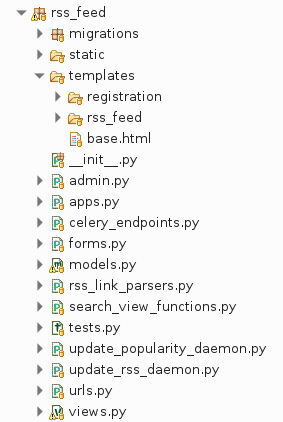
\includegraphics[scale=0.6,keepaspectratio=true]{./images/project_tree.png}
	\caption{Árbore de módulos do aplicativo web.}
	\label{fig:project_tree}
\end{figure}


\subsection{Capa Modelo}

Á hora de definir esta cuestión, tratáronse de respectar as regras do modelo relacional de bases de datos, porén, fixeronse algunhas excepcións motivadas por esixencia da elección do framework Django:

\begin{itemize}
	\item Claves primarias subrogadas: Django encárgase da identificación das tuplas engadindo ás táboas un campo numérico enteiro de incremento automático. Isto utilizarase en todas as táboas sen excepción.
	
	\item Relación 1-1: Como se ve no diagrama Entidade-Relación da figura \ref{fig:diagrama_er}, existe unha relación 1-1 entre a entidade User e a súa entidade feble UserProfile. O motivo da existencia desta última é que se decidiu utilizar a entidade de usuario nativa de Django, co cal fíxose necesaria unha nova táboa para cubrir os atributos de usuario necesarios especificamente para o proxecto. 
\end{itemize}

No diagrama Entidade-Relación da figura \ref{fig:diagrama_er} pódense ver as táboas empregadas sen incluir aquelas automáticamente xeradas para o correcto funcionamento de Django e Celery a excepción da xa mencionada User. Por motivos de claridade, non se incluíron os atributos agás aqueles adicionais nas táboas correspondentes ás relacións N-N.

A estrutura da BD tradúcese na aplicación ás clases definidas no paquete models.py que se ve na figura \ref{fig:clase_models}. Por claridade, nese diagrama de clases só se incluíron os atributos máis representativos ou explicativos das relacións entre clases.

\begin{figure}[h]
	\centering
	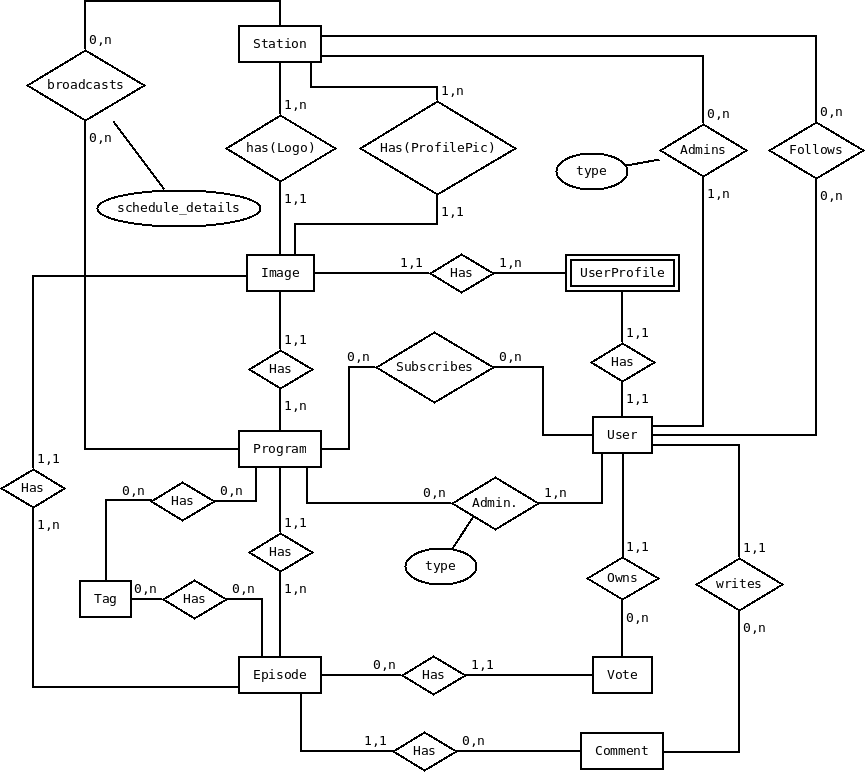
\includegraphics[scale=0.5,keepaspectratio=true]{./images/ER_diagrama.png}
	\caption{Diagrama Entidade-Relación da Base de Datos.}
	\label{fig:diagrama_er}
\end{figure}

\begin{figure}[h]
	\centering
	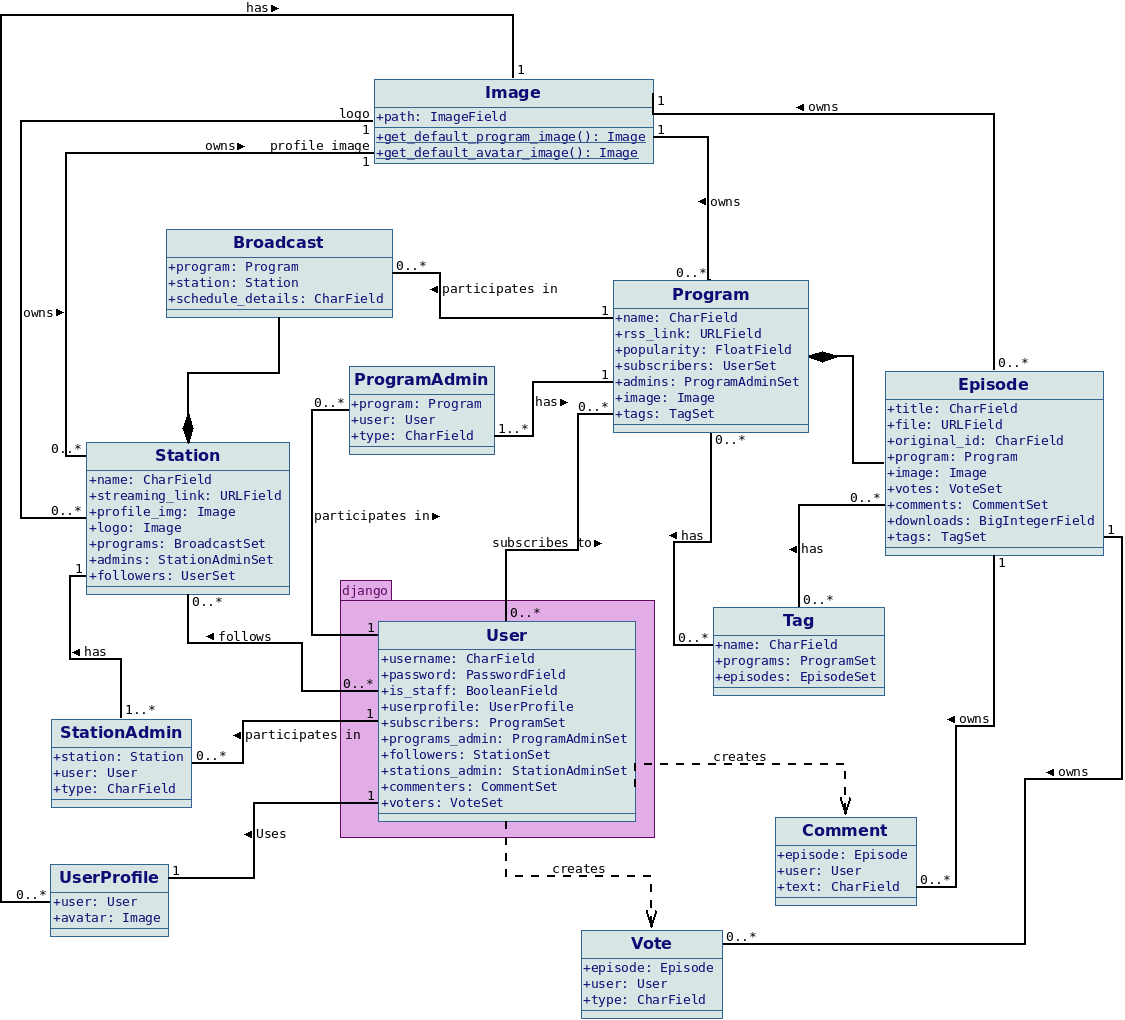
\includegraphics[scale=0.4,keepaspectratio=true]{./images/class_diagram.png}
	\caption{Diagrama de clases da capa modelo.}
	\label{fig:clase_models}
\end{figure}


\subsubsection{Usuarios}

Os usuarios están definidos por dúas táboas: User e UserProfile que se corresponden coas clases User, do paquete django.contrib.auth.models, e UserProfile, definida polo desenvolvedor e, polo tanto, includida no módulo models.py. Esta segunda considerámola coma feble de User pois a existencia dun perfil está vencellada de xeito ineludible á existencia dun usuario (ver figura \ref{fig:diagrama_er}). Esta entidade auxiliar contén os atributos de usuario: avatar, descrición e localizción. Non se utiliza para máis nada.

A clase User inclúe os atributos necesarios para a autenticación: username, email e password, quedando este último encriptado en base de datos mediante o algoritmo PBKDF2. De entre os campos utilizados para o funcionamento de Django, cómpre destacar is\_staff, que é o que concede acceso do usuario ao panel de administración do aplicativo que provee o propio framework (como se mencionou no apartado \ref{django})

Outros atributos de User reflectidos na figura \ref{fig:clase_models} coma followers ou station\_admins son engadidos automáticamente polo framework ao declarar as relacións coa fin de facilitar a navegación entre clases.


\subsubsection{Programas e episodios}

Entendemos, neste sistema, un programa coma un produto radiofónico do cal se publican entregas periodicamente. Están almacenados na táboa Program da base de datos. Os programas teñen, entre outros atributos, un nome, unha descrición, unha imaxe, un conxunto de categorías (táboa Tag) e un enlace a un ficheiro RSS dado polo usuario.

A subscrición dos usuarios aos programas modelouse coma unha relación N-N. As instancias de Program poden acceder ao conxunto dos seus subscritores mediante o atributo subscribers.

Episodio é como chamamos ás entregas dun programa. Cada un ten, entre outros atributos, un enlace a un ficheiro de audio que será o que se poña a disposición dos usuarios na interface, un resumo, unha imaxe e un conxunto de etiquetas (tags). Un episodio ten que formar parte de 1 e só 1 programa. Se un programa é borrado, os episodios deixan de ter sentido no sistema e son borrados en cascada. Debido ao anterior, considérase a relación destas clases coma unha composición.


\subsubsection{Votos e comentarios}

Nunha primeira aproximación ao deseño da base de datos, entendéronse estas dúas entidades coma simples relacións N-N entre as entidades Episode e User. Porén, decidiuse finalmente que representan conceptos de seu que non perden o sentido semántico fóra da relación e, polo tanto, modeláronse coma entidades (Vote e Comment nos diagramas \ref{fig:diagrama_er} e \ref{fig:clase_models}).

O atributo type de Vote serve para lle dar significado ao voto: Positivo, negativo ou neutro.


\subsubsection{A entidade Station}

Identifícanse coa entidade Station os colectivos aos que se poidan asociar os programas: Emisoras de radio por ondas, emisoras de radio por internet ou canles de podcasting. O atributo mais destacable de Station é o de streaming\_link, que garda o enlace á canle de emisión por internet da emisora que será logo utilizado polo reproductor na web. Este campo pode ser nulo para aqueles colectivos que non dispoñan de emisión en directo.  

A emisión dos programas por parte das emisoras queda modelada coma unha relación N-N entre Program e Station á que chamamos broadcasts. Engadiuse o atributo adicional de schedule\_details, un campo de texto para os detalles de emsión: Horario, periodicidade... A clase correspondente en models.py é Broadcast. Dada a natureza de Station coma aglutinador de programas e dado que non ten sentido a existencia dunha emisión sen emisora, entendeuse que a relación entre Broadcast e Station é de composición. 


\subsubsection{Administración de contido}

Existe unha relación N-N entre os usuarios e as emisoras e unha semellante entre os usuarios e os programas: A de administración. Entendemos esta coma a posibilidade de editar, actualizar e borrar os contidos preexistentes. Isto queda reflectido nas clases ProgramAdmin e StationAdmin. As súas instancias relacionan, respectivamente, aos usuarios cos programas e emisoras que poden administrar e establecen os permisos de administración que posúen, estes últimos, expresados polo atributo type.

Tanto para a administración de emisoras como de Programas, existen dous roles: Propietario e administrador. O propietario ten permisos completos: Edición, actualización, borrado e xestión de administradores. O administrador só ten permisos de edición e actualización.  

Nótese que tal relación de administración non existe no caso dos episodios. Isto débese a que, ao ser engadidos automaticamente segundo a información recibida polo ficheiro RSS do programa (explicado máis en detalle na sección \ref{rss_parser_section}), non son editables. Aquelas opcións que poidan afectar en bloque aos episodios dun programa considéranse xa opcións do programa.

Os superusuarios do sistema, pola súa parte, poden editar e borrar calquera contido mediante ferramentas de Django coma o panel de administración ou o IPython shell.


\subsection{Capa Vista}

A capa vista é na que se atopa a lóxica funcional do aplicativo. Fai uso dos obxectos da capa modelo para, ou ben extraer e compñer os datos que serán enviados ao cliente ou ben recoller os datos enviados desde o cliente para facer as conseguintes modificacións na base de datos. O módulo central desta capa é views.py. Nel, defínense funcións e clases que reciben un obxecto de Django HttpRequest e unha serie de parámetros opcionais e, tras realizar as operacións necesarias, retornan un obxecto HttpResponse.

Un obxecto HttpRequest contén metadatos da petición que se executou desde o cliente: Información da sesión do usuario, tipo de petición (GET, POST...), datos necesarios para os posibles \say{middlewares} e datos que o cliente envía a través dos formularios. 

Os middlewares, en Django, son plugins que alteran globalmente a entrada e saída do procesamento das peticións e as respostas. O framework oferta certa variedade de plugins de serie e a posibilidade de crear middlewares propios. Comentaranse os utilizados no capítulo de Implementación.

Un obxecto HttpResponse contén os datos que han de ser devoltos ao cliente, incluíndo a páxina á que se ha de redirixir ao usuario por causa da petición. Django require gardar os datos nun dicionario clave-valor ao que chama context. Esas claves valerán para acceder aos valores no template á hora de renderizar a resposta.

A decisión de a qué instancia ou función se lle pasa o obxecto HttpRequest tómase en base á url destino enviada polo cliente xunto co propio obxecto. É necesario manter un módulo que relacione as urls coas funcións e clases correspondentes á operación a realizar. Comunmente en Django e tamén neste proxecto, este ficheiro chámase urls.py.

\begin{figure}[H]
	\centering
	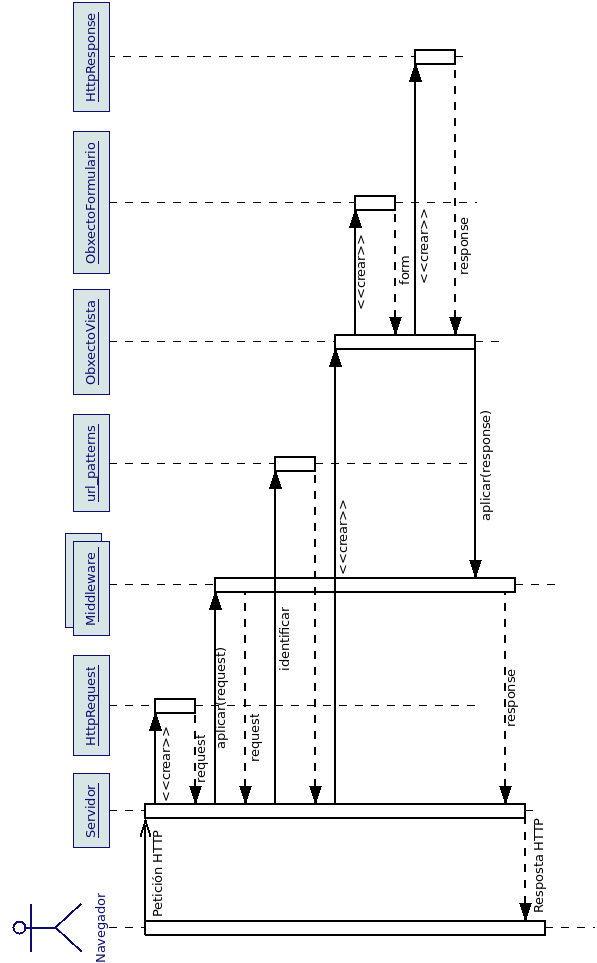
\includegraphics[scale=0.6,keepaspectratio=true]{./images/secuencia_vista_v.png}
	\caption{Esquema do funcionamento das vistas.}
	\label{fig:vista}
\end{figure} 

Na figura \ref{fig:vista} amósase un esquema do funcionamento da capa vista. Para unha maior claridade, condensáronse as distintas clases de middleware nun único paso do diagrama. Tamén nesa figura pode verse unha referencia ao obxectos Form de Django que son utilizados neste proxecto. Estes obxectos consisten nunha abstracción a obxecto de Python da información procedente dos formularios despregados no template e dos contedores de dita información (selectores, caixas de texto...). O seu uso é opcional, pero simplifican a definición valores por defecto e a validación dos datos. 




\subsubsection{Engadir contido}
\label{rss_parser_section}

Explicarase en detalle esta vista por ser, a posibilidade de que os usuarios engadan os seus propios programas e os episodios, a parte principal deste proxecto. Un usuario, pode engadir un programa e todos os seus episodios simplemente proporcionándolle ao aplicativo o enlace ao seu ficheiro de RSS.

\begin{figure}[h]
	\centering
	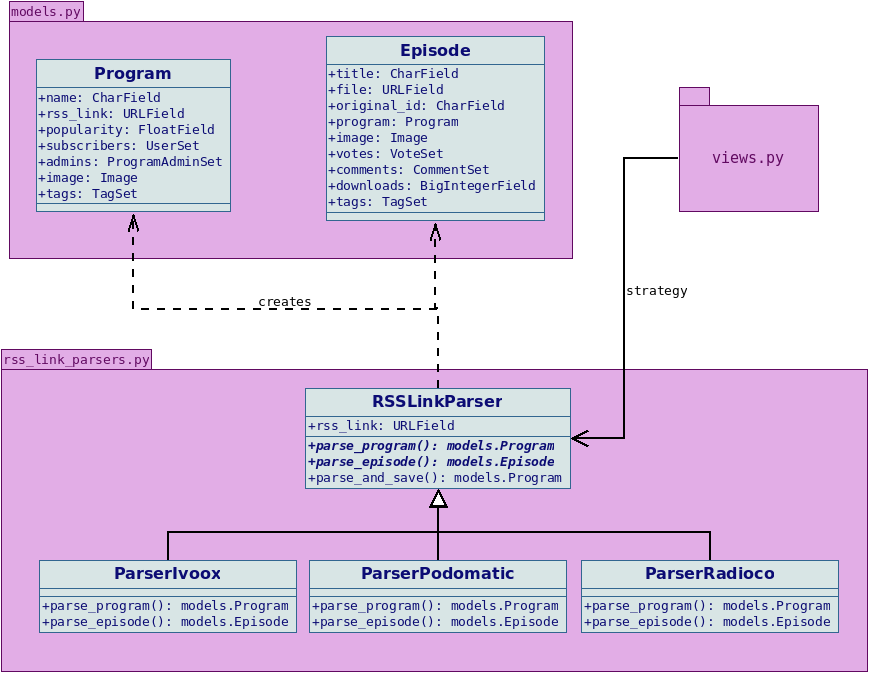
\includegraphics[scale=0.45,keepaspectratio=true]{./images/strategy.png}
	\caption{Patrón Estratexia utilizado para o procesamento de RSS.}
	\label{fig:strategy}
\end{figure}

A función de vista encargada de realizar este traballo recibe o obxecto de request e carga os datos deste nun formulario de Django. Unha vez validado, accede ao ficheiro RSS e extrae os datos do programa e os episodios. Enfrontámonos aquí a unha limitación do proxecto: Non existe un estándar de campos de RSS. Distintos servidores de podcasting poden ter distintos formatos.

Debido a isto, debía deseñarse o sistema de xeito que puidésemos contar con distintos algoritmos de interpretación do RSS e, de cara a unha continuación do desenvolvemento, que engadir novos algoritmos fose sinxelo. De modo que se decidiu aplicar o patrón de deseño \say{estratexia}, como se ve no diagrama \ref{fig:strategy}. A superclase, RSSLinkParser, implementa o método parse\_and\_save, encargado da creación das novas instancias. Esta función utiliza os métodos de lectura da información de programa e episodio, pero deixa a súa implementación ás clases fillas. Actualmente, o proxecto soporta 3 tipos ficheiro RSS dos máis populares entre os usuarios obxectivo.


\subsection{Capa Template}

A capa template define a forma na que os datos obtidos na capa vista serán amosados ao usuario e tamén os métodos de entrada de datos que poremos a disposición deste. A idea xeral foi a dunha interface na que os datos simples (atributos) se amosan en forma de lista e os complexos (Entidades) en forma de cuadrícula. Cada elemento desa cuadrícula representa un programa, episodio ou emisora da forma representada na figura \ref{fig:grella} e constitúe un enlace á páxina de detalles desa entidade.

\begin{figure}[H]
	\centering
	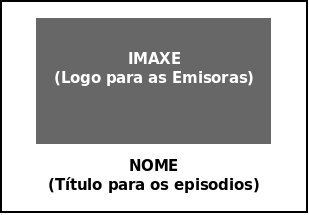
\includegraphics[scale=0.6,keepaspectratio=true]{./images/grella.png}
	\caption{Esquema dun elemento da cuadrícula.}
	\label{fig:grella}
\end{figure}

Pensando no uso da web en dispositivos móbiles, o número de elementos por fila da cuadrícula varía dependendo do tamaño da pantalla. Aquelas páxinas divididas de xeito horizontal (esquerda e dereita)  pasan a verticais (arriba e abaixo) pois considerase o \say{scroll} vertical máis cómodo para o usuario destes dispositivos. 

Todas as páxinas levan unha cabeceira amosando a información transversal á páxina: Un enlace á portada, botón de inicio/peche de sesión, unha caixa de procura por texto e máis o selector de linguaxe. 

A continuación coméntase brevemente as diferentes partes da interface:

\subsubsection{Portada}

Pensouse na portada coma unha páxina que ofreza información breve e xeral que o usuario queira consultar con máis frecuencia, por exemplo, as novidades nas súas subscricións e o acceso rápido ás súas emisoras favoritas. Tamén, pensando nos usuarios anónimos, considerouse engadir información de interese xeral coma os episodios máis recentes ou os programas máis \say{populares}, concepto que se explica na sección \ref{daemon_desenho}.

Na figura \ref{fig:index1_p} amósase un primeiro borrador desta páxina. Móstrase a información dos programas e os episodios en forma de grella na parte esquerda e das emisoras en forma de lista no lado dereito. Isto cambia nos pequenos dispositivos, onde a información das emisoras pasa a situarse na parte máis baixa da páxina.

\begin{figure}[h]
	\centering
	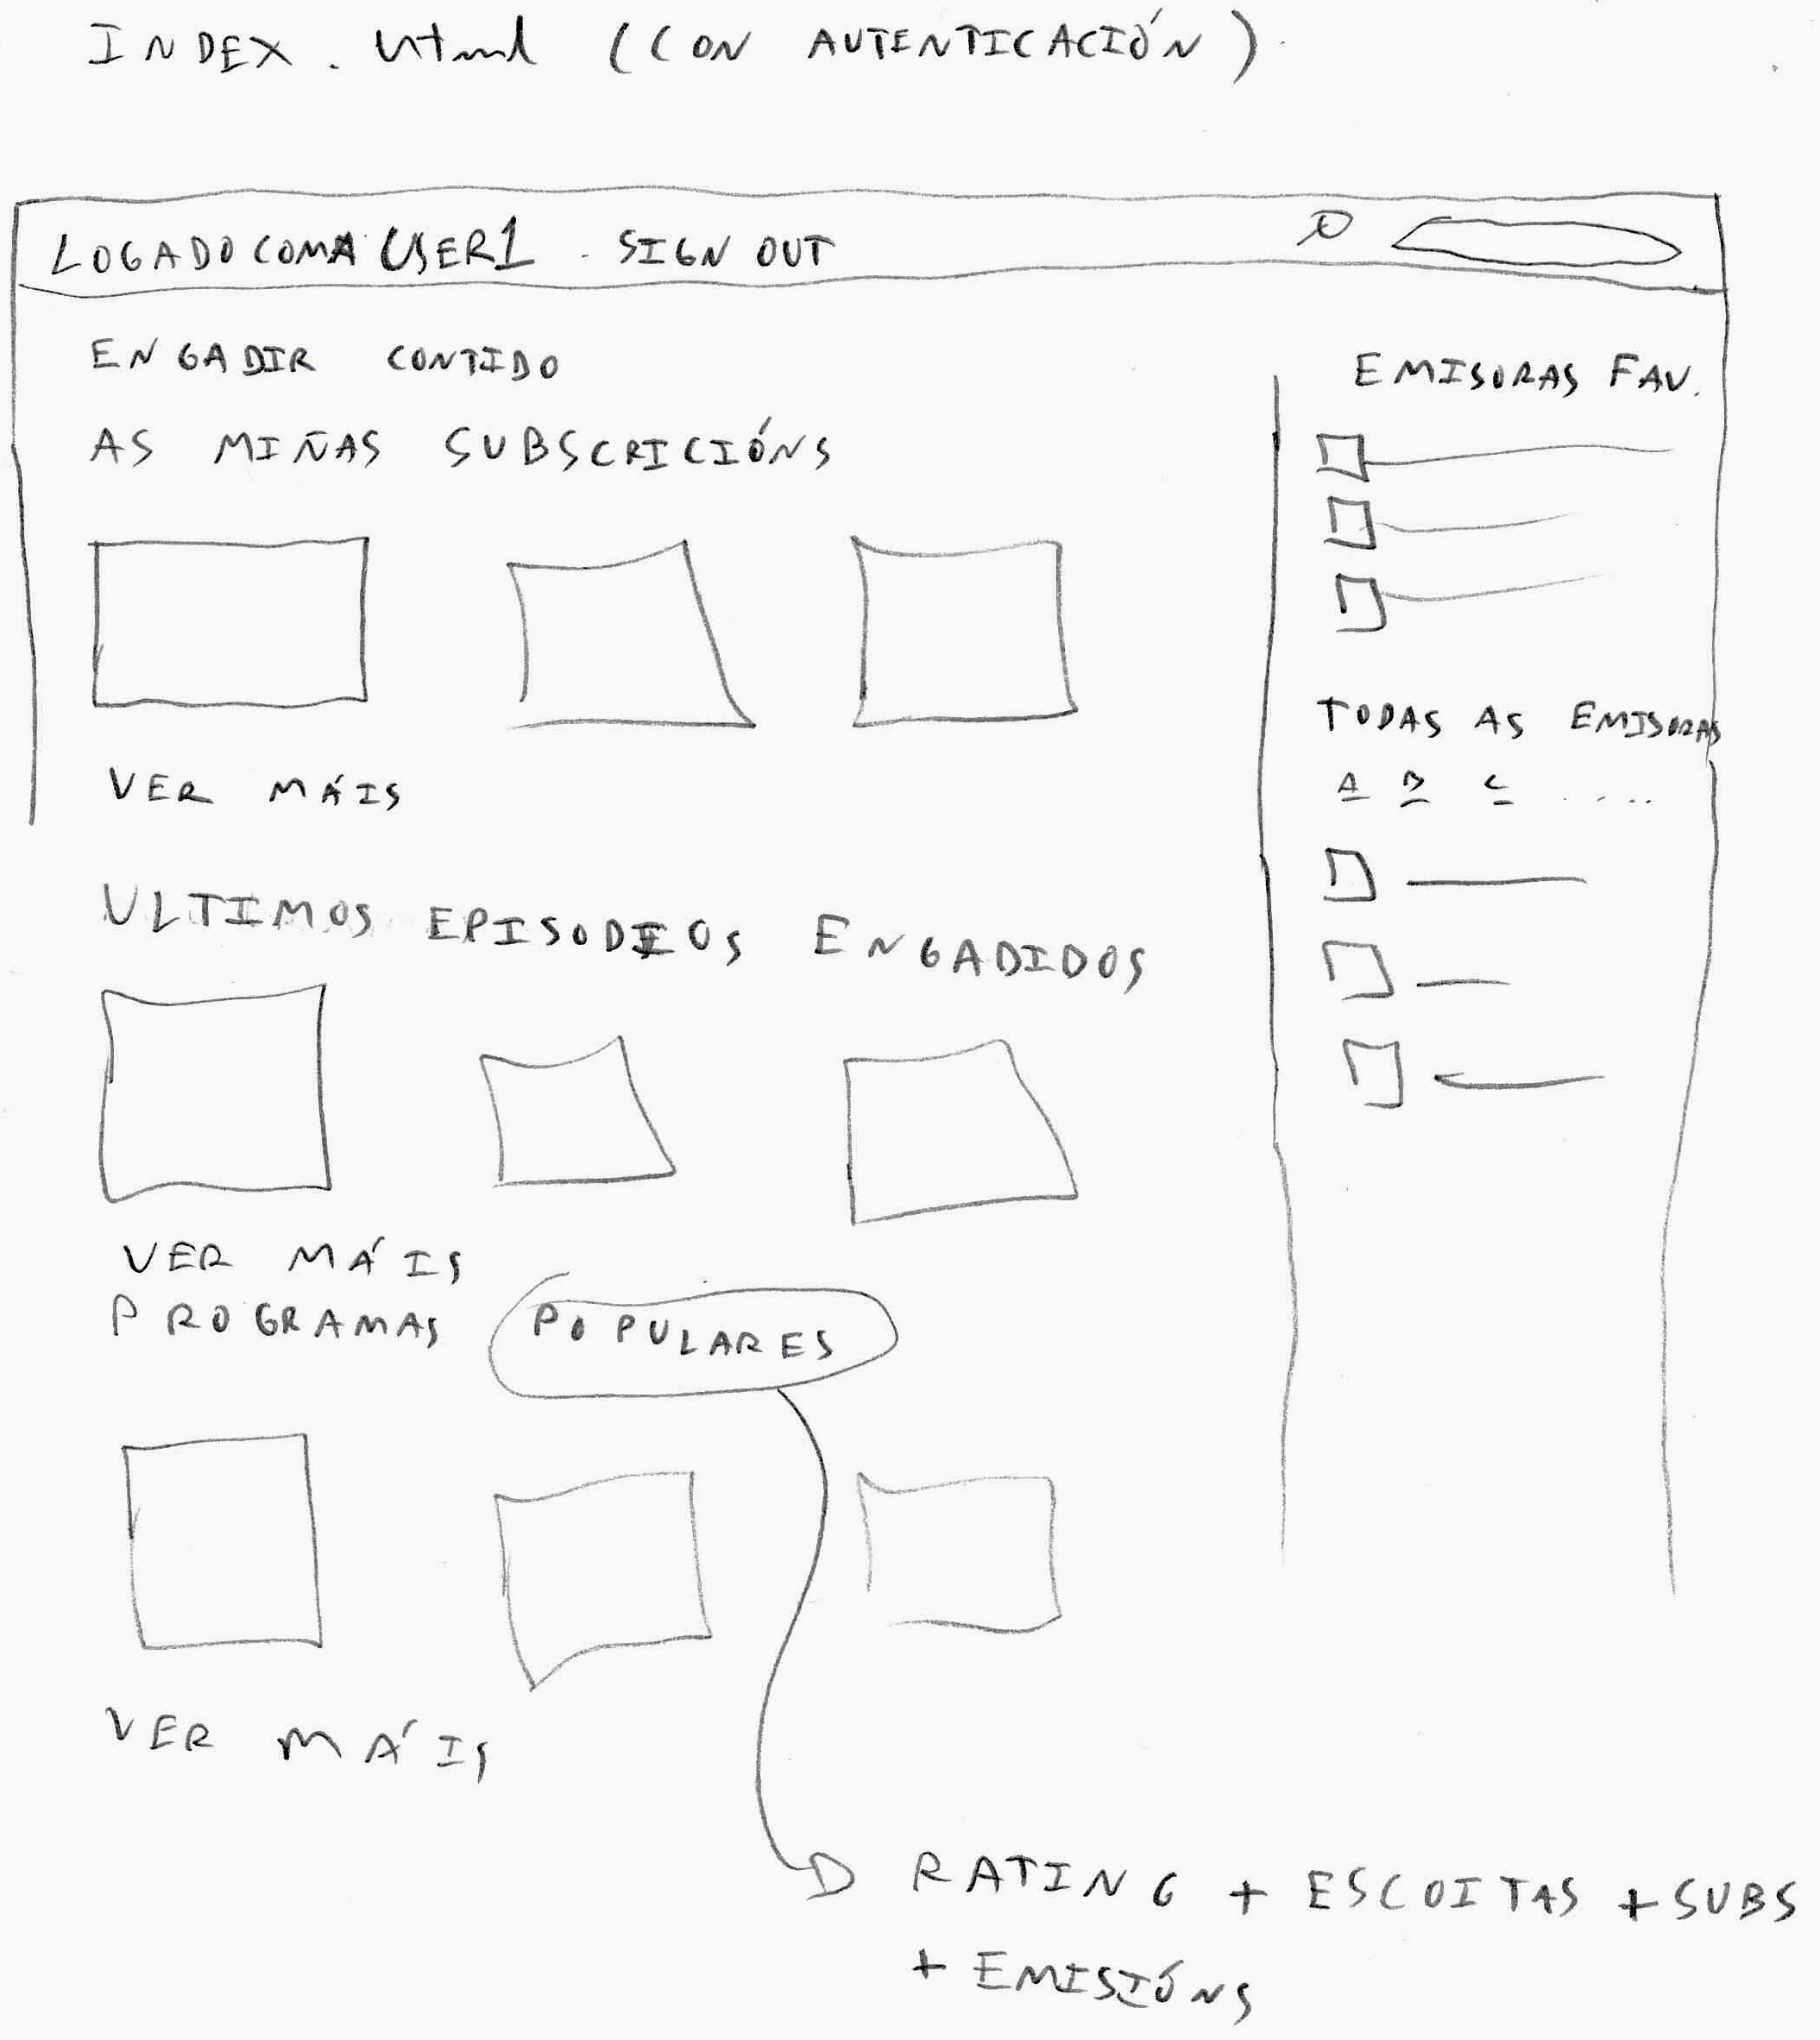
\includegraphics[scale=0.2,keepaspectratio=true]{./images/index1_p.png}
	\caption{Extracto do borrador do deseño da interface. Portada.}
	\label{fig:index1_p}
\end{figure}


\subsubsection{Páxinas de detalle}

Ás páxinas de detalle son aquelas onde se amosa a información completa dunha instancia dalgunha das 4 grandes clases deste proxecto: Usuario, emisora, programa e episodio. Tamén debería dar acceso á páxina de edición de ter, o usuario, permisos para iso.

Na figura \ref{fig:program1_p} amosamos un borrador da páxina de detalles de programa que nos ha valer coma exemplo xeral: Encabézase coa imaxe da instancia e o seu nome. Debaixo, lístanse os seus atributos incluíndo o reprodutor de audio para os casos de emisora e episodio. Finalmente, as cuadrículas dos obxectos cos que se relacionan.

A máis distinta sería, se cadra, a de episodio. Esta incluiría ao final unha sección de comentarios en lugar dunha grella de obxectos.

\begin{figure}[h]
	\centering
	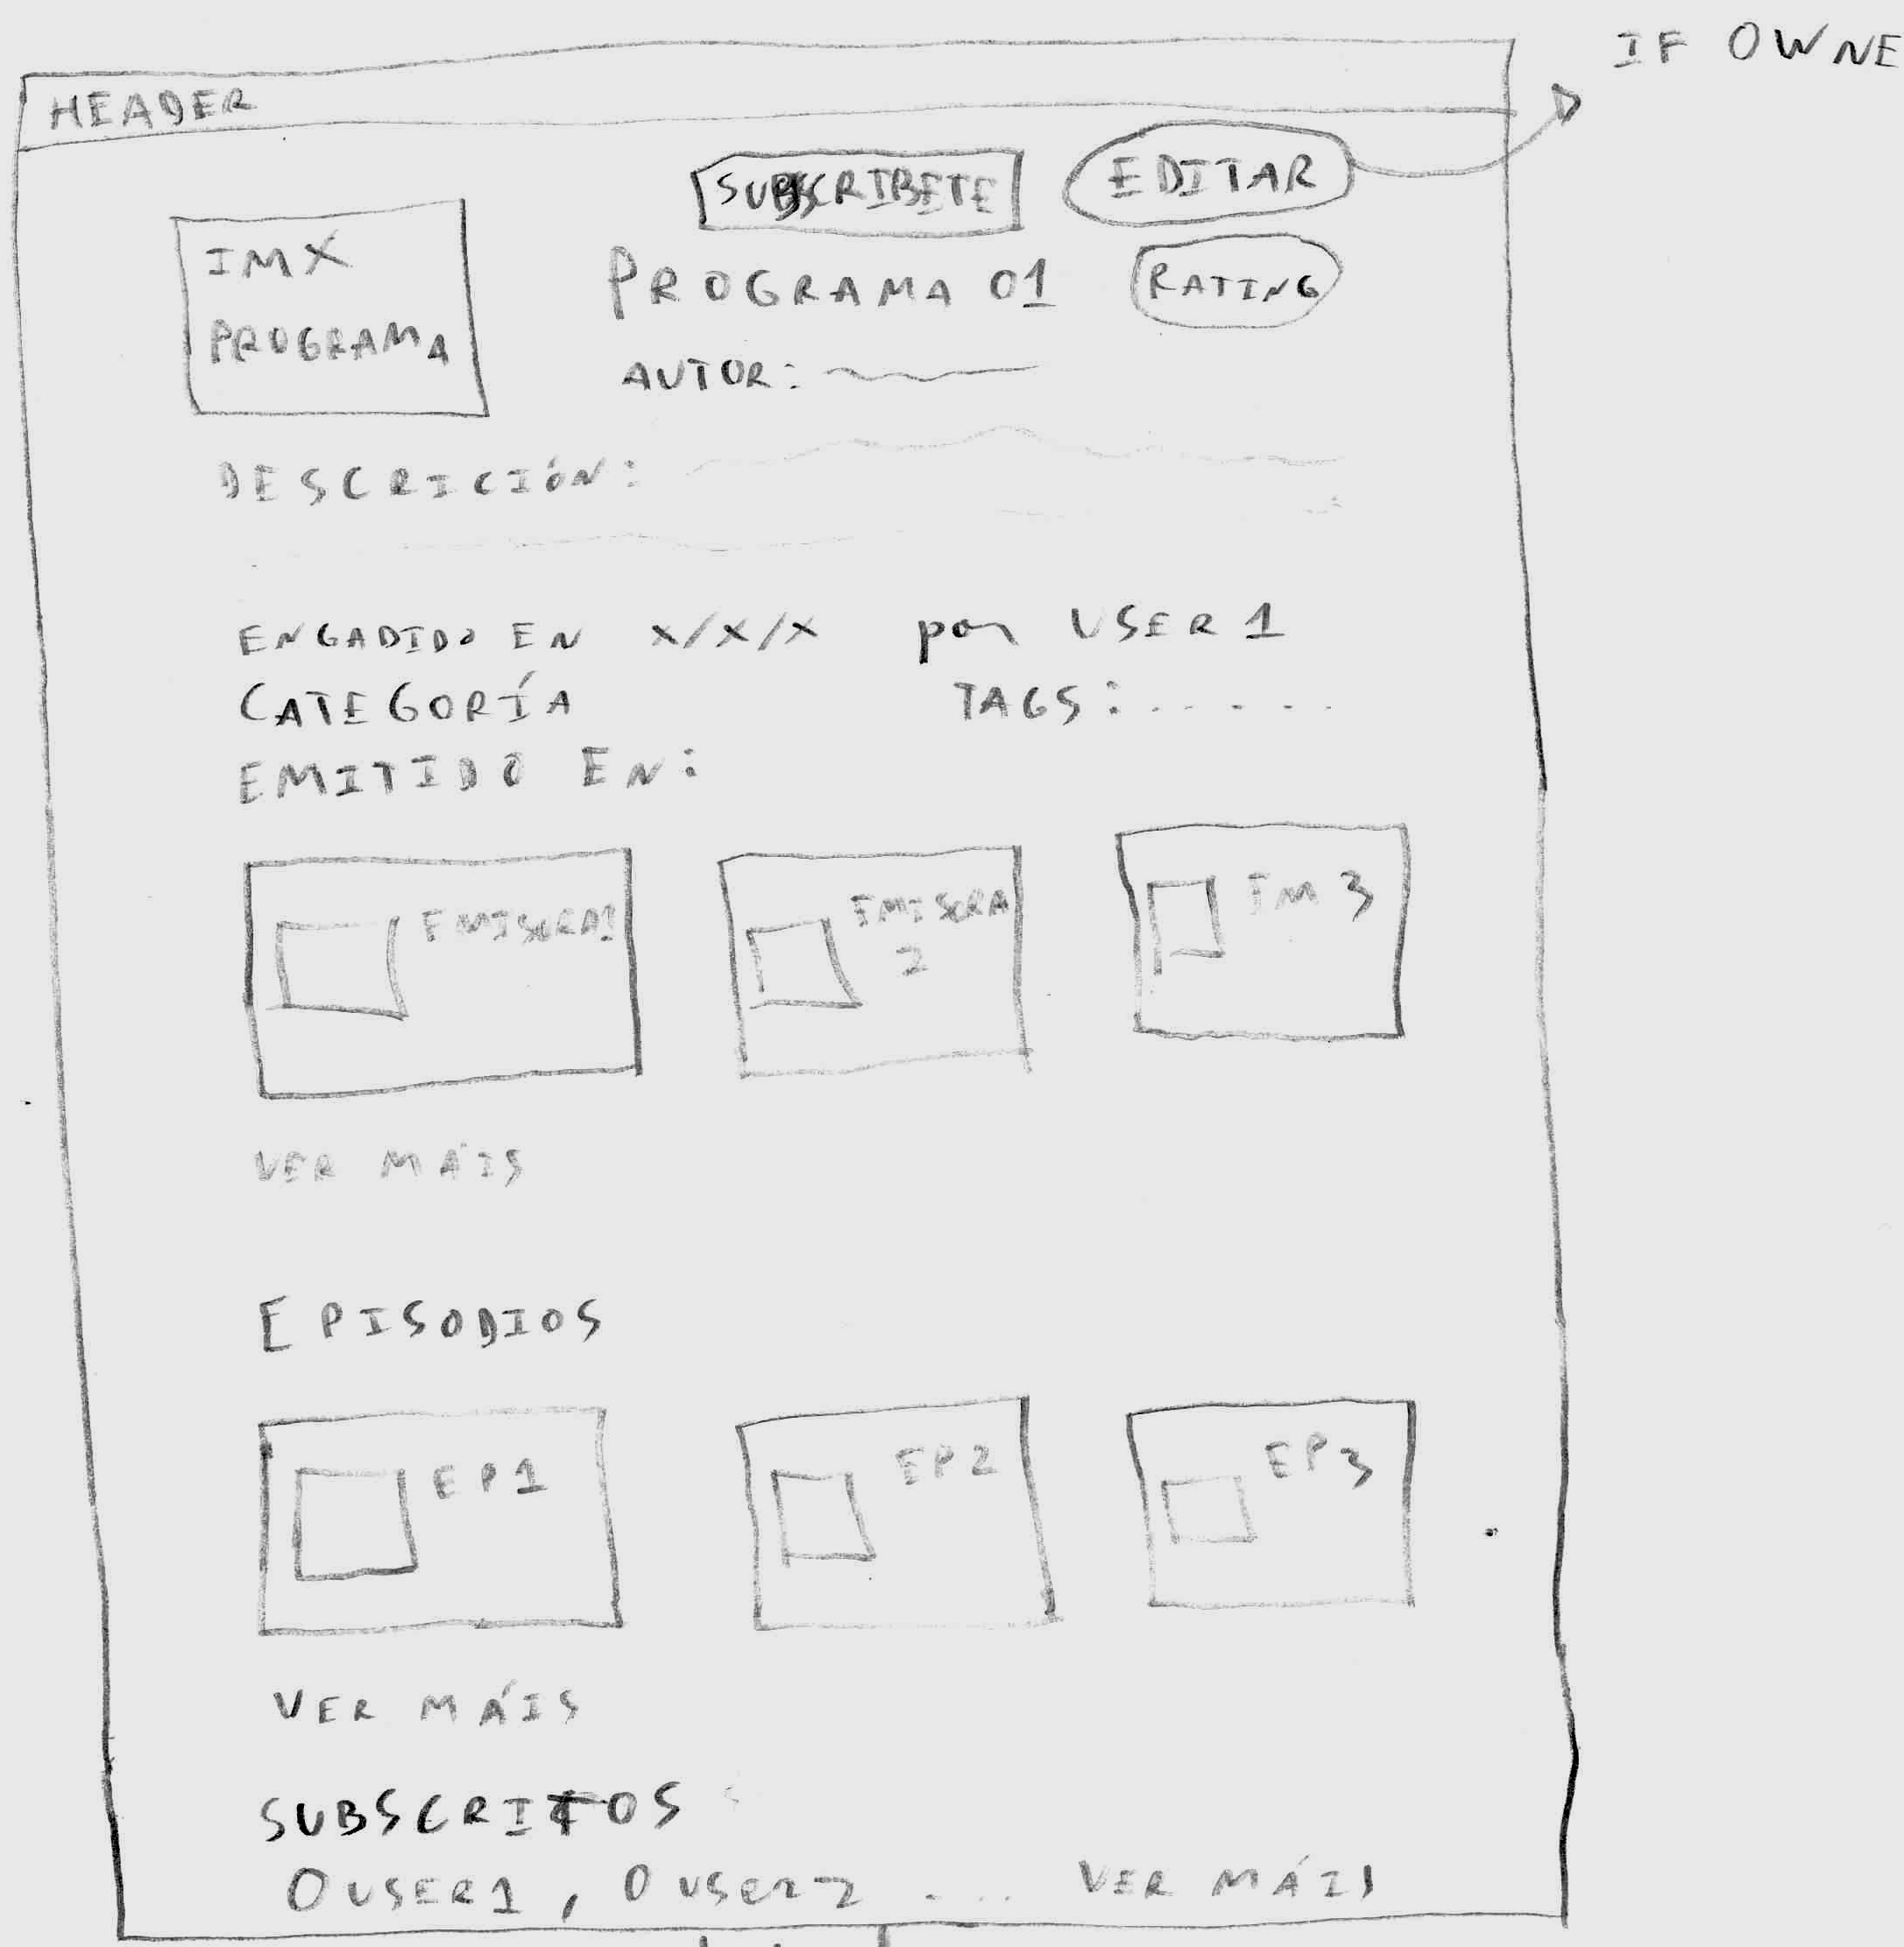
\includegraphics[scale=0.2,keepaspectratio=true]{./images/program1_p.png}
	\caption{Extracto do borrador do deseño da interface. Detalles de programa.}
	\label{fig:program1_p}
\end{figure}


\section{Actualización dos datos}
\label{daemon_desenho}
[Por Facer]
  \chapter[Implementación]{
  \label{chp:implementacion}
  Implementación
}
\minitoc
\newpage

En el presente capítulo se prestará atención a la arquitectura de la aplicación,
es decir, a los bloques de construcción del programa. Los componentes son:
paquetes, librerías, frameworks, \textit{APIs}, etc descritos en términos de
módulos, clases, funciones y algoritmos. En esencia, se trata del software y de
la organización del código fuente. Se mostrarán fragmentos de código del
software implementado con los aspectos más significativos. Esta parte de la
documentación técnica es de gran importancia para comprender el proyecto.


\section{Organización del código fuente}

El código fuente de todo el proyecto, incluida la presente memoria realizada en
\LaTeX, se ha gestionando en Git, usando el flujo de trabajo Git-Flow. Se ha
estructurado el código fuente de la siguiente forma:

  \chapter[Planificación]{
  \label{chp:plan}
  Planificación
}
\minitoc
\newpage

Neste capítulo explicarase a planificación do traballo realizado e a avaliación de custes.  

\section{Iteracións}

Como se explicou no capítulo \ref{chp:metodoloxia}, o desenvolvemento executouse de  de forma iterativa e incremental onde unha iteración son os obxectivos a cumprir entre dúas reunións co cliente. Ao ser isto un proxecto de final de carreira, contarase o tempo entre as sesións de revisión de progresos entre o director do proxecto e o alumno.

\subsection{Reunión inicial}

Produciuse un encontro con membros de Cuac FM (a radio comunitaria da Coruña) e a URCM onde se entrou en contacto cos usuarios finais do proxecto a realizar. A URCM (Unión de Radios Comunitarias de Madrid) está composta por unha serie de emisoras independentes e con programas de seu; todos eles listados nunha sección da web (ver figura \ref{fig:urcm}) que á súa vez da acceso ao directorio dos ficheiros de audio (aos que a partir de agora nos referiremos coma \say{audios}) publicados por ditas emisoras. Esta sección da web, pese a súas limitacións, leva funcionando uns anos e resultou ser moi positiva para a redifusión dos programas por distintos colectivos.

\begin{figure}[h]
	\centering
	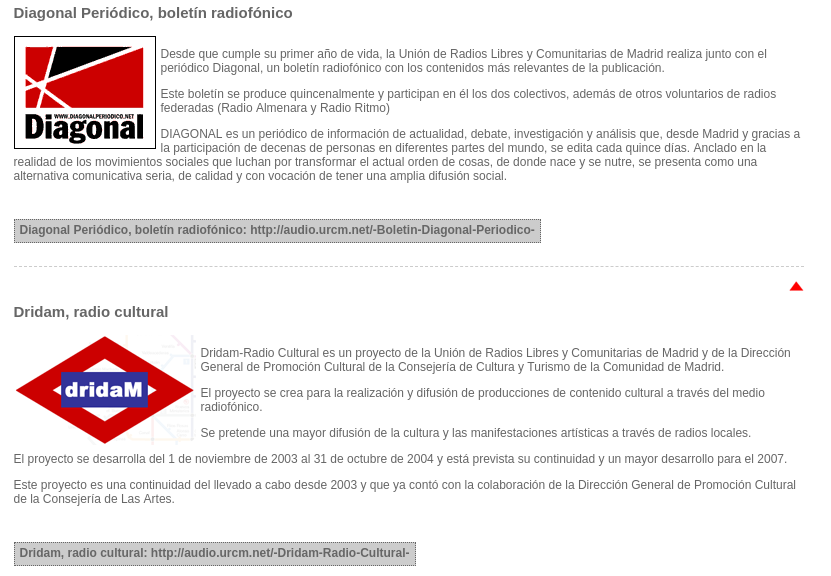
\includegraphics[scale=0.55,keepaspectratio=true]{./images/urcm.png}
	\caption{Sección de audios da web da URCM que inspira o proxecto.}
	\label{fig:urcm}
\end{figure}

Inspirados nesta idea, propúxose crear unha ferramenta semellante, esta vez para a ReMC (Red de medios comunitarios), unha federación de medios comunitarios do Estado Español. Definíronse uns requirimentos iniciais, máis centrados naquel entón na
redifusión e a organización que na escoita.

\subsubsection{Requirimentos primitivos}

A seguinte lista é unha transcrición das notas tomadas durante esa primeira reunión:

\begin{itemize}
	\item Os usuarios dos sistema son as propias emisoras.
	\item As emisoras teñen que poder engadir audios.
	\item As emisoras poden acceder aos audios das outras.
	\item As emisoras teñen que poder saber quen está a emitir os seus programas.
\end{itemize}



  \chapter[Probas do sistema]{
  \label{chp:test}
  Probas do sistema
}
\minitoc
\newpage

Neste capítulo explicarase o proceso de probas ao que se someteu o sistema desenvolvido. 

\section{Plan de probas}

Durante as primeiras fases do desenvolvemento utilizouse a técnica \textbf{TDD} (ver capítulo \ref{chp:metodoloxia} sobre metodoloxía) polo que se comezou realizando \textbf{probas de unidade automatizadas} para as clases do modelo de datos e as do módulo rss\_link\_parsers.py.

As \textbf{probas de integración} comezaron á vez que o desenvolvemento das funcións e clases de vista do módulo views.py. Son tamén tests de unidade pero utilizando un simulador de peticións GET e POST.

Finalmente, realizouse un conxunto de \textbf{tests de aceptación} de xeito manual. Utilizáronse para validar o correcto funcionamento da \textbf{interface}.


\section{Probas de unidade}

Son aquelas que verifican o \textbf{correcto funcionamento individual das compoñentes}. Para realizar este tipo de probas, cómpre definir un entorno independente para cada unha de xeito que os resultados das anteriores non inflúan nas posteriores. Os casos de proba están automatizados. Isto fai posible executalos cando se fagan cambios no código coa fin de detectar a aparición de efectos non desexados. O código correspondente pode atoparse no ficheiro \textbf{tests.py} incluído no proxecto (ver figura \ref{fig:project_tree})

Utilizouse a biblioteca \textit{django.test} de Django, a cal, mediante o uso do paquete \textit{unittest} estándar de Python, permite a escritura das probas de unidade. Defínense, para isto, conxuntos de casos de proba en forma de clase que ha ser herdeira da \textbf{clase TestCase}, incluída na biblioteca. Confecciónanse, a continuación, as probas en forma de métodos cuxo nome ha levar o prefixo "test".

Para asegurar a independencia entre probas, Django creará unha \textbf{base de datos temporal} que será borrada automaticamente unha vez os tests finalicen, independentemente do seu éxito. Isto implica que cada instancia filla de TestCase teña que popular a base de datos coma paso previo á execución dos tests, podendo isto facerse en cada proba ou declarando un \textbf{método setUp}.


\begin{lstlisting}[language=Python, caption=Probas de unidade dos metodos de Program, label=lst:programtest]
class ProgramModelTests(TestCase): 


	def setUp(self):
	
		rssl = 'http://dummy_link.xml'
		p_image = Image.objects.create(name='p_image1',path='path/to/p_image1')
		
		p1 = Program.objects.create(name='TestProgram1',rss_link=rssl,image=p_image)
		
		u1 = User.objects.create(username='userp1')
		u2 = User.objects.create(username='userp2')
		User.objects.create(username='userp3')
		
		p1.programadmin_set.create(user=u1,type=ADMT_OWNER[0])
		p1.programadmin_set.create(user=u2,type=ADMT_ADMIN[0])
		
		t1 = Tag.objects.create(name='pt1',times_used=1)
		t2 = Tag.objects.create(name='pt2',times_used=2)
		
		p1.tag_set.add(t1)
		p1.tag_set.add(t2)
	
	
	def test_check_user_is_admin(self):
	
		p1 = Program.objects.get(name='TestProgram1')
		u1 = User.objects.get(username='userp1')
		u2 = User.objects.get(username='userp2')
		u3 = User.objects.get(username='userp3')
		
		self.assertTrue(p1.check_user_is_admin(u1,ADMT_OWNER[0]))
		self.assertFalse(p1.check_user_is_admin(u1,ADMT_ADMIN[0]))
		self.assertTrue(p1.check_user_is_admin(u2,ADMT_ADMIN[0]))
		self.assertFalse(p1.check_user_is_admin(u2,ADMT_OWNER[0]))
		self.assertFalse(p1.check_user_is_admin(u3))
	
	
	def test_delete(self):
	
		p1 = Program.objects.get(name='TestProgram1')
		p1_id = p1.id
		img_id = p1.image.id
		
		p1.delete()
		
		p2 = list(Program.objects.filter(pk=p1_id))
		self.assertEqual(p2,[])
		
		img2 = list(Image.objects.filter(pk=img_id))
		self.assertEqual(img2,[])
		
		t1 = Tag.objects.get(name='pt1')
		t2 = Tag.objects.get(name='pt2')
		
		self.assertEqual(t1.times_used,0)
		self.assertEqual(t2.times_used,1)

\end{lstlisting}
 

O código amosado no exemplo \ref{lst:programtest} é o utilizado nas probas de unidade da clase \textbf{Program}. Primeiro, o método \textit{setUp} crea na base de datos temporal o programa \textit{p1}, 3 usuarios dos cales lle asigna 2 coma administradores e máis 2 tags que tamén lle asigna. Nótese que se utiliza un método de creación propio dun obxecto imaxe, iso é posible porque xa ten a súa propia proba de unidade executada anteriormente no mesmo ficheiro. O código xa probado pasa a considerarse seguro e pode ser utilizado nos tests seguintes.

O primeiro test comproba que o método \textit{check\_user\_is\_admin(user,[type])} de Program responda correctamente á pregunta de se o usuario dado é administrador dese programa e cos permisos especificados. O segundo comproba se o método de borrado borra tamén a imaxe asignada e fai decrecer o contador de uso dos tags. Probas semellantes se fixeron para as clases do módulo models.py que posúen métodos propios.


\begin{lstlisting}[language=Python, caption=Probas de unidade dos metodos de ParserIvoox, label=lst:ivooxtest]
class ParserIvooxRSSLPTests(TestCase):


	def initialize_test(self):
	
		RSS_file = TEST_AUX_FILE_PATH + 'hasta-los-kinders_original.xml'
		feed_dict = feedparser.parse(RSS_file)
		u1 = User.objects.create(username='userRSSLP1')
		
		return ParserIvoox(RSS_file,u1),feed_dict
	
	
	def test_get_entry_list(self):
	
		rlp,fd = self.initialize_test()
		el = rlp.get_entry_list(fd)
		
		self.assertIsInstance(el,list)
		self.assertIsInstance(el[0],dict)
	
	
	def test_parse_program(self):
	
		program_web = 'http://www.ivoox.com/podcast-hasta-los-kinders_sq_f14062_1.html'
		rlp,fd = self.initialize_test()
		
		p1 = rlp.parse_program(fd)
		
		self.assertEqual(p1.name,'Hasta Los Kinders')
		self.assertEqual(p1.language,'es-ES')
		self.assertEqual(p1.original_site,program_web)
		self.assertEqual(p1.rss_link_type,IVOOX_TYPE[0])
	
	
	def test_parse_episode(self):
	
		rlp,fd = self.initialize_test()
		
		#Expected info
		exp_titlte = 'CiudadanoKinders: Como hacer un monologo'
		exp_pub_date = datetime.datetime(2010, 9, 17, 20, 45, 24, tzinfo=pytz.utc)
		exp_file = 'http://www.ivoox.com/ciudadanokinders-como-hacer-monologo_mf_368919_feed_1.mp3'
		exp_web = 'http://www.ivoox.com/ciudadanokinders-como-hacer-monologo-audios-mp3_rf_368919_1.html'
		exp_original_id = 'http://www.ivoox.com/368919'
		
		p1 = rlp.parse_program(fd)
		entry_dict = rlp.get_entry_list(fd)[0]
		
		e1 = rlp.parse_episode(entry_dict,p1)
		
		self.assertIsInstance(e1,Episode)
		self.assertEquals(e1.title,exp_titlte)
		self.assertEquals(e1.publication_date,exp_pub_date)
		self.assertEquals(e1.file,exp_file)
		self.assertEquals(e1.original_site,exp_web)
		self.assertEquals(e1.original_id,exp_original_id)
	
	
	# From superclass
	def test_parse_and_save(self):
		
		rlp,_ = self.initialize_test()
		
		p1 = rlp.parse_and_save()
		self.assertIsInstance(p1,Program)
		
		p1_id = p1.id
		p2 = list(Program.objects.filter(pk=p1_id))
		self.assertNotEqual(p2,[])
		
		p2 = p2[0]
		
		self.assertEqual(p2.tag_set.count(),1)
		self.assertEqual(p2.tag_set.all()[0].name,'comedy')
		self.assertIsInstance(p2.image,Image)
		
		
		self.assertEqual(p2.episode_set.count(),20)
		
		e1 = p2.episode_set.filter(title='CiudadanoKinders: Como hacer un monologo')
		self.assertNotEqual(e1,[])
		
		e1 = e1[0]
		self.assertIsInstance(e1,Episode)
		
		self.assertEquals(e1.image,p2.image)
		
		# Clean copied image
		p2.image.delete()
\end{lstlisting}   

No exemplo \ref{lst:ivooxtest} atópase o código que valeu para probar o funcionamento dun dos \textbf{intérpretes de RSS} do módulo rss\_link\_parser.py (ver sección \ref{rss_parser_section}), concretamente o correspondente aos ficheiros co formato de Ivoox.  Tanto con este coma cos outros \say{parsers} probáronse as subrutinas auxiliares e máis os métodos \textit{parse\_program} e \textit{parse\_episode}. No amosado, inclúese tamén o test da función \textit{parse\_and\_save} herdada da superclase.

Para realizar as anteriores probas utilizáronse \textbf{ficheiros RSS reais} descargados a disco local. Dado que o obxectivo último desta clase é a creación de obxectos a partir da información do RSS, as probas enfócanse en comprobar se o gardado en base de datos coincide co esperado.


\begin{lstlisting}[language=Python, caption=Probas de unidade do proceso de actualización de popularidade, label=lst:popdaemon]
class UpdatePopularityDaemonTests(TestCase):


	def setUp(self):
	
		u1 = User.objects.create(username='userUPD1')
		u2 = User.objects.create(username='userUPD2')
		s1 = Station.objects.create(name='RadioTest2')
		
		RSS1 = TEST_AUX_FILE_PATH + 'hasta-los-kinders_original.xml'
		rlp = ParserIvoox(RSS1,u1)
		hlk = rlp.parse_and_save()
		
		hlk_ep1 = hlk.episode_set.all()[0]
		hlk_ep1.vote_set.add(Vote.objects.create(type=LIKE_VOTE[0],user=u1,episode=hlk_ep1))
		
		hlk_ep2 = hlk.episode_set.all()[1]
		hlk_ep2.vote_set.add(Vote.objects.create(type=LIKE_VOTE[0],user=u1,episode=hlk_ep2))
		
		hlk_ep3 = hlk.episode_set.all()[2]
		hlk_ep3.vote_set.add(Vote.objects.create(type=DISLIKE_VOTE[0],user=u1,episode=hlk_ep3))
		hlk_ep3.vote_set.add(Vote.objects.create(type=LIKE_VOTE[0],user=u2,episode=hlk_ep3))
		
		RSS2 = TEST_AUX_FILE_PATH + 'falacalado_podomatic.xml'
		rlp = ParserPodomatic(RSS2,u1)
		fc = rlp.parse_and_save()
		fc.subscribers.add(u1)
		fc.broadcast_set.add(Broadcast.objects.create(station=s1,program=fc,schedule_details='Friday 21:00'))
		
		fc_ep1 = fc.episode_set.all()[0]
		fc_ep1.downloads = 1000
		fc_ep1.save()
	
	
	def test_update_pop_rating_all_programs(self):
		
		hlk = Program.objects.get(name='Hasta Los Kinders')
		fc = Program.objects.get(name="fala calado's podcast")
		
		self.assertEqual(hlk.rating,50)
		self.assertEqual(fc.popularity,0)
		
		#Ignore 365 days limitation
		update_pop_rating_all_programs(days=0)
		
		hlk2 = Program.objects.get(name='Hasta Los Kinders')
		fc2 = Program.objects.get(name="fala calado's podcast")
		
		exp_pop = program_popularity_formula(1,1,0,1000)
		
		self.assertEqual(hlk2.rating,75)
		self.assertEqual(fc2.popularity,exp_pop)
\end{lstlisting}

As funcións que compoñen os procesos executados polo servidor para actualizar os programas (ver sección \ref{daemon_desenho}) tamén foron sometidos a probas. No exemplo \ref{lst:popdaemon} vese o código do test de unidade do proceso que actualiza os campos de \textit{rating} (cualificación) e \textit{popularity} (popularidade) dos programas. Para iso, créase en \textit{setUp} os programas \textit{hlk} e \textit{fc} mediante os parsers de Ivoox e Podomatic (previamente probados) respectivamente. Despois, manipúlanse as características valorables para o rating no primeiro e as valorables para popularity no segundo.

Ao comezar o test, compróbase se os valores de ámbolos dous atributos son os iniciais, logo executase o código de actualización e, finalmente, compróbase se os valores cambiaron da forma esperada.

\section{Probas de integración}

Son aquelas que serven para \textbf{verificar o traballo conxunto de distintas compoñentes}. Estes casos de test, por regra xeral, tratan de probar as conexións entre compoñentes ignorando o funcionamento interno\cite{tests}.

No módulo views.py atópanse as funcións que reciben os datos entrantes e pasan as respostas ao cliente. Para probalas foi necesario o uso da \textbf{clase Client}, dispoñible na biblioteca de Django utilizada para os tests. Esta clase interactúa co sistema a modo de navegador web sinxelo permitindo simular operacións de GET e POST, ver a cadea redirección entre os distintos templates e comprobar que os datos presentes no contexto son os axeitados.

\begin{lstlisting}[language=Python, caption=Fragmento das probas da vista index, label=lst:index]
class IndexViewTests(TestCase):


	@classmethod
	def setUpTestData(cls):
	
		u1 = User.objects.create(username='userIV1')
		
		RSS1 = TEST_AUX_FILE_PATH + 'hasta-los-kinders_original.xml'
		rlp = ParserIvoox(RSS1,u1)
		hlk = rlp.parse_and_save()
		hlk.popularity = 10 # Check if first
		hlk.save()
		
		RSS2 = TEST_AUX_FILE_PATH + 'falacalado_podomatic.xml'
		rlp = ParserPodomatic(RSS2,u1)
		rlp.parse_and_save()
		
		# Total of 10 + 2 programs
		for i in range(1,11):
		
		rssl = 'http://dummy_link_iv_' + str(i) + '.xml'
		pname = 'ProgramIV_' + str(i)
		Program.objects.create(name=pname,rss_link=rssl)
		
		# Create 30 stations
		for i in range(1,31):
		
		sname = 'StationIV_' + str(i)
		Station.objects.create(name=sname)


    def test_view_uses_correct_template(self):

		resp = self.client.get(reverse('rss_feed:index'))
		self.assertEqual(resp.status_code, 200)
		
		self.assertTemplateUsed(resp, 'rss_feed/index.html')


	def test_program_list(self):

		resp = self.client.get(reverse('rss_feed:index'))
		self.assertEqual(resp.status_code, 200)
		
		self.assertEqual( len(resp.context['program_list']),4)
		self.assertTrue(resp.context['program_list'].has_next())
		self.assertFalse(resp.context['program_list'].has_previous())
		
		p1 = resp.context['program_list'][0]
		p2 = Program.objects.get(name='Hasta Los Kinders')
		self.assertEqual(p1,p2)
		
		resp = self.client.get('/rss_feed/?p_page=3')
		self.assertEqual(resp.status_code, 200)
		
		self.assertEqual( len(resp.context['program_list']),4)
		self.assertFalse(resp.context['program_list'].has_next())
		self.assertTrue(resp.context['program_list'].has_previous())
	
\end{lstlisting}


No exemplo \ref{lst:index} vénse algunhas probas realizadas para a vista de \textit{index}, que se corresponde coa páxina principal da aplicación. Créanse primeiro, na función de clase \textit{setUpTestData}, 12 programas e 20 emisoras co obxectivo de comprobar que o contexto está a pasar o número deles correcto, na orde correcta e cos datos axeitados a cerca da paxinación. Isto realízase no segundo test, o do método \textit{test\_program\_list}, só para o caso dos programas (as emisoras tamén se proban, pero incluílo semella redundante). O primeiro test, \textit{test\_view\_uses\_correct\_template}, comproba que se accede á vista index a través do template axeitado.

\begin{lstlisting}[language=Python, caption=Fragmento das probas da vista add\_content, label=lst:add_content]
class AddContentViewTests(TestCase):


	def setUp(self):
	
		u2 = User.objects.create(username='userIV2')
		u2.set_password('12345678A')
		u2.save()
	
	
	def test_login(self):
	
		self.client.login(username='userIV2',password='12345678A')
		resp = self.client.get(reverse('rss_feed:add_content'))
		
		self.assertEqual(resp.status_code, 200)
		self.assertEqual(str(resp.context['user']), 'userIV2')
		
		self.assertTemplateUsed(resp, 'rss_feed/add_content.html')
	
	
	def test_add_station(self):
	
		self.client.login(username='userIV2',password='12345678A')
		
		form_station = {'form_station-name': ['StationIV1'], 'form_station-logo': [''], 'form_station-profile_img': [''], 
		'form_station-broadcasting_method': ['fm'], 'form_station-broadcasting_area': [''], 
		'form_station-broadcasting_frequency': [''], 'form_station-streaming_link': [''], 
		'form_station-description': [''], 'form_station-website': [''], 'form_station-location': ['']}
		
		self.client.post(reverse('rss_feed:add_content'),  form_station)
		
		s1 = Station.objects.get(name='StationIV1')
		
		self.assertIsInstance(s1,Station)
		self.assertEqual(s1.logo,Image.get_default_program_image())
\end{lstlisting}


Aquelas vistas que requiran que o usuario estea identificado tamén poden ser probadas, como se ve no exemplo \ref{lst:add_content}. O primeiro caso proba que o login funciona e que se utiliza o template correcto. O segundo, proba a inserción dunha nova emisora a través do formulario que se enviaría desde a interface web.


\section{Probas de aceptación}

O código puramente de \textbf{frontend} (Javascript, HTML...) foi probado de xeito manual e non automatizado. Tamén se contou cun usuario alleo ao proxecto para realizar un pequeno conxunto de probas.

  \chapter[Conclusións]{
  \label{chp:conclusiones}
  Conclusións
}
\minitoc
\newpage

Neste capítulo porase en balance o traballo realizado e darase unha breve guía de melloras que poderían implementarse no futuro.

A aplicación web presentada nesta memoria cumpre cos obxectivos iniciais do proxecto (ver sección \ref{obxectivos}) 

\begin{itemize}
	\item Creouse un portal web que da \textbf{acceso a ficheiros de audio}, ou ben mediante streaming por Internet, ou ben por descarga directa, estando estes aloxados nun servidor alleo.
	\item Implementáronse funcionalidades para que os \textbf{usuarios engadan o seu propio contido}. Poden engadir as súas emisoras ou programas de forma manual. No caso dos episodios, son creados automaticamente mediante os algoritmos de lectura de ficheiros RSS. Estes mesmos algoritmos, agrupan os arquivos de audio por programa e categoría.
	\item Puxéronse a disposición dos usuarios \textbf{ferramentas de procura} de contidos por texto e máis por etiqueta. 
	\item Habilitouse, para os usuarios, un \textbf{sistema de subscrición} aos programas e de seguimento das emisoras.
	\item Deseñouse un esquema de roles e permisos para facilitar a \textbf{colaboración entre os usuarios} nas tarefas de xestión de contidos.
	\item Logrouse o anterior utilizando ferramentas e bibliotecas de software libre, o cal permite que \textbf{o software teña unha licenza de software libre} que satisfai os requisitos da Free Software Foundation.
\end{itemize}


A medida que o traballo avanzaba, fóronse intuíndo novas necesidades que os usuarios poderían ter. Destas, implementáronse as seguintes:

\begin{itemize}
	
	\item Panel de administración: Provese dunha interface web de administración para que un superusuario do sistema poida manipular os datos presentes na base de datos.
	
	\item Visualización por méritos: Creouse o concepto de \say{popularidade} dos programas. Canto máis popular sexa un programa, máis posibilidades terá de saír en portada e aparecerá antes nos resultados de busca.
	
	\item Comentarios e votos: Os usuarios poden dar \say{feedback} aos autores dos programas mediante votos e comentarios nos episodios.
	
	\item Limitación de redifusión dos programas: Un dos fins deste proxecto é facilitar o intercambio de programas por parte de distintas emisoras, porén, poden darse situacións nas que se queira limitar esa posibilidade. As \say{Opcións de compartición} poden ser seleccionadas no panel de xestión do programa.
	
\end{itemize}


Persoalmente, considero que se desenvolveu unha ferramenta útil para os medios do terceiro sector. A aplicación web creada dá resposta a unha serie de necesidades reais que coñezo de primeira man, non so polos contactos con membros deste tipo de medios, senón tamén pola miña experiencia persoal colaborando en Cuac FM. O aumento das sinerxias entre colectivos é unha necesidade de supervivencia para estes e creo que este proxecto é un modesto aporte.   


\section{Coñecementos acadados}

Durante os meus anos coma estudante e coma profesional, o deseño web nunca foi unha predilección debido ao caóticas que me resultaban as ferramentas de desenvolvemento de \textbf{frontend}. Forzarme a utilizar JavaScript e afondar no meu coñecemento de CSS e HTML foi unha forma de tirar eses prexuízos e diversificar os meus coñecementos.

Aprender \textbf{Django} foi un aspecto moi positivo deste traballo, pois completa bastante a miña experiencia de uso de Python, linguaxe que me esperta especial interese.

O proxecto tamén me valeu para refrescar conceptos teóricos de \textbf{enxeñaría do software} (metodoloxías, xestión de proxectos, patróns de deseño...) e como aplicalos.


\section{Futuros traballos}

A continuación, exponse unha lista de melloras que se poderían levar a cabo no futuro:

\begin{itemize}
	
	\item \textbf{Rediseño da interface de xestión de Programas e Emisoras:} Tras amosar a interface a xente allea ao proxecto, parece que a configuración actual das ferramentas de entrada de datos nesas vistas poden levar a certa confusión.
	
	\item \textbf{Enriquecer información de emisión:} O horario de emisión dun programa por unha emisora é información en texto. Poderíase modelar ese dato de xeito que o sistema puidese responder a preguntas coma: \say{Que programas se emiten os luns?}, \say{Que programa se está a emitir agora?}
	
	\item \textbf{Crear caixa de mensaxes para os usuarios:} Actualmente, os usuarios poden ver os novos episodios das súas subscricións na portada, pero estaría ben que se lles avisase cunha mensaxe directa. Poderíanse enviar mensaxes para máis eventos, por exemplo: \say{A emisora \textit{RadioX} quere emitir o teu programa \textit{ProgramaY}}
	
	\item \textbf{Melloras en seguridade:} O rexistro de usuario podería ter un CAPTCHA para evitar a un atacante crear usuarios de xeito automatizado. Tamén se podería pedir un número de teléfono aos usuarios para implementar unha \say{verificación de dous pasos}.
\end{itemize}

  
  \appendix
  \chapter[Apéndice]{
  \label{chp:dicionario}
  Dicionario de datos
}
Neste apéndice figura, por orde alfabética, unha descrición dos modelos de datos utilizados. Inclúense so as entidades definidas de forma propia, non aquelas dadas polo framework (por exemplo, User). Do mesmo xeito, non se inclúen os atributos automaticamente definidos pola declaración relacións en Django. 

\textbf{Broadcast:} Clase que representa a relación N-N de emisión entre programas e emisoras.

\begin{longtable}{|p{3cm}|p{3cm}|p{8cm}|}
	\hline
	\rowcolor{gray!50}
	Atributo & Tipo & Descrición\\
	\hline
	@\textbf{id} & Serial & Clave primaria\\
	\hline
	\textbf{program} & ForeignKey & Clave foránea da entidade Program\\
	\hline
	\textbf{station} & ForeignKey & Clave foránea da entidade Station\\	
	\hline
	\textbf{schedule\_details} & Char(100) & Texto do comentario\\
	\hline
\end{longtable}


\textbf{Comment:} Entidade que garda os comentarios que os usuarios deixan nos episodios.

\begin{longtable}{|p{3cm}|p{3cm}|p{8cm}|}
	\hline
	\rowcolor{gray!50}
	Atributo & Tipo & Descrición\\
	\hline
	@\textbf{id} & Serial & Clave primaria\\
	\hline
	\textbf{episode} & ForeignKey & Clave foránea da entidade Episode\\
	\hline
	\textbf{user} & ForeignKey & Clave foránea da entidade User\\	
	\hline
	\textbf{text} & Text & Texto do comentario\\
	\hline
	\textbf{publication\_date} & DateTime & Data de publicación (GMT)\\
	\hline
	\textbf{removed} & Boolean & Marcado coma borrado\\
	\hline
\end{longtable}



\textbf{Episode:} Entidade que garda cada unha das entregas (episodios) dos programas.

\begin{longtable}{|p{3cm}|p{3cm}|p{8cm}|} 
	\hline
	\rowcolor{gray!50}
	Atributo & Tipo & Descrición\\
	\hline
	@\textbf{id} & Serial & Clave primaria\\
	\hline
	\textbf{program} & ForeignKey & Clave foránea da entidade Program\\
	\hline
	\textbf{title} & Char(200) & Título do episodio\\	
	\hline
	\textbf{summary} & Text & Resumo do episodio\\
	\hline
	\textbf{publication\_date} & DateTime & Data de publicación (GMT)\\
	\hline
	\textbf{insertion\_date} & DateTime & Data de inserción na base de datos (GMT)\\
	\hline
	\textbf{file} & URL & Enlace ao ficheiro de audio\\
	\hline
	\textbf{file\_type} & Char(40) & Enlace ao ficheiro de audio\\
	\hline
	\textbf{downloads} & BigInt & Contador de descargas e escoitas do episodio\\
	\hline
	\textbf{original\_id} & Char(200) & Id do episodio no sistema orixinal de almacenamento\\
	\hline
	\textbf{original\_site} & URL & Páxina do episodio no sistema orixinal de almacenamento\\
	\hline
	\textbf{removed} & Boolean & Marcado coma borrado\\
	\hline
	\textbf{image} & ForeignKey & Clave foránea da entidade Image\\
	\hline
	\textbf{votes} & ManyToMany & Referencia ás instancias de Vote relacionadas\\
	\hline
	\textbf{comments} & ManyToMany & Referencia ás instancias de Comment relacionadas\\
	\hline
	
\end{longtable}


\textbf{Program:} Entidade que garda os programas engadidos polos usuarios.

\begin{longtable}{|p{3cm}|p{3cm}|p{8cm}|}
	\hline
	\rowcolor{gray!50}
	Atributo & Tipo & Descrición\\
	\hline
	@\textbf{id} & Serial & Clave primaria\\
	\hline
	\textbf{image} & ForeignKey & Clave foránea da entidade Image\\
	\hline
	\textbf{name} & Char(200) & Nome do programa\\	
	\hline
	\textbf{description} & Text & Texto descritivo sobre o programa\\
	\hline
	\textbf{creation\_date} & DateTime & Data de inserción na base de datos (GMT)\\
	\hline
	\textbf{author\_email} & Email & Correo electrónico do autor do programa\\
	\hline
	\textbf{author} & Char(200) & Autor orixinal extraído do ficheiro RSS\\
	\hline
	\textbf{language} & Char(10) & Código de linguaxe do programa\\
	\hline
	\textbf{rss\_link} & URL & Enlace ao ficheiro RSS do programa\\
	\hline
	\textbf{rss\_link\_type} & Char[ivoox $|$ radioco $|$ podomatic] & Tipo de RSSLinkParser utilizado na súa creación\\
	\hline
	\textbf{rating} & PositiveSmall Integer[0:100] & Cualificación calculada para o programa\\
	\hline
	\textbf{original\_site} & URL & Enlace ao podcast orixinal\\
	\hline
	\textbf{popularity } & Float & Popularidade calculada para o programa\\
	\hline
	\textbf{website} & URL & Páxina web do programa\\
	\hline
	\textbf{sharing\_options} & Char[share\_free $|$ no\_share] & Condicións de compartición\\
	\hline
	\textbf{comment \_options} & Char[enable $|$ disable] & Opción de activar ou desactivar comentarios\\
	\hline
	\textbf{subscribers} &  ManyToMany & Referencia ás instancias de User relacionadas. Representa os subscritores do programa\\
	\hline
	\textbf{admins} &  ManyToMany & Referencia ás instancias de ProgramAdmin relacionadas\\
	\hline
\end{longtable}


\textbf{ProgramAdmin:} Clase que representa a relación N-N de administración entre programas e usuarios.

\begin{longtable}{|p{3cm}|p{3cm}|p{8cm}|}
	\hline
	\rowcolor{gray!50}
	Atributo & Tipo & Descrición\\
	\hline
	@\textbf{id} & Serial & Clave primaria\\
	\hline
	\textbf{program} & ForeignKey & Clave foránea da entidade Program\\
	\hline
	\textbf{user} & ForeignKey & Clave foránea da entidade User\\	
	\hline
	\textbf{type} & Char[owner $|$ admin] & Permisos do usuario sobre o programa\\
	\hline
	\textbf{date} & DateTime & Data na que se concedeu o permiso (GMT)\\
	\hline
\end{longtable}


\textbf{Station:} Entidade que garda os colectivos de emisión (radios por ondas, radios por internet, canles de podcast...)

\begin{longtable}{|p{3cm}|p{3cm}|p{8cm}|}
	\hline
	\rowcolor{gray!50}
	Atributo & Tipo & Descrición\\
	\hline
	@\textbf{id} & Serial & Clave primaria\\
	\hline
	\textbf{logo} & ForeignKey & Clave foránea da entidade Image para o logotipo da emisora\\
	\hline
	\textbf{profile\_img} & ForeignKey & Clave foránea da entidade Image para a imaxe de cabeceira do perfil\\
	\hline
	\textbf{name} & Char(200) & Nome da emisora\\	
	\hline
	\textbf{broadcasting \_method} & Char[RadioFM $|$ RadioAM $|$ RadioDigital $|$ TVChannel $|$ RadioInternet $|$ PodcastingChannel $|$ Others] & Método de emisión dos programas \\
	\hline
	\textbf{broadcasting \_area} & Char(200) & Área de emisión (No caso de RadioFM, RadioAM e RadioDigital)\\
	\hline
	\textbf{broadcasting \_frequency} & Char(50) & Frecuencia de emisión (No caso de RadioFM, RadioAM e RadioDigital)\\
	\hline
	\textbf{streaming\_link} & URL & Enlace á emisión en directo por streaming\\
	\hline
	\textbf{website} & URL & Enlace á páxina web do colectivo\\
	\hline
	\textbf{location} & Char(200) & Localización da emisora\\
	\hline
	\textbf{programs} &  ManyToMany & Referencia ás instancias de Broadcast relacionadas\\
	\hline
	\textbf{admins} &  ManyToMany & Referencia ás instancias de ProgramAdmin relacionadas\\
	\hline
	\textbf{followers} &  ManyToMany & Referencia ás instancias de User relacionadas. Representa os seguidores da emisora.\\
	\hline
\end{longtable}

\textbf{StationAdmin:} Clase que representa a relación N-N de administración entre emisoras e usuarios.

\begin{longtable}{|p{3cm}|p{3cm}|p{8cm}|}
	\hline
	\rowcolor{gray!50}
	Atributo & Tipo & Descrición\\
	\hline
	@\textbf{id} & Serial & Clave primaria\\
	\hline
	\textbf{station} & ForeignKey & Clave foránea da entidade Station\\
	\hline
	\textbf{user} & ForeignKey & Clave foránea da entidade User\\	
	\hline
	\textbf{type} & Char[owner $|$ admin] & Permisos do usuario sobre a emisora\\
	\hline
	\textbf{date} & DateTime & Data na que se concedeu o permiso (GMT)\\
	\hline
\end{longtable}	


\textbf{Tag:}  Entidade que garda os etiquetas de categoría dadas polos ficheiros RSS.

\begin{longtable}{|p{3cm}|p{3cm}|p{8cm}|}
	\hline
	\rowcolor{gray!50}
	Atributo & Tipo & Descrición\\
	\hline
	@\textbf{id} & Serial & Clave primaria\\
	\hline
	\textbf{name} & Char(50) & Nome do tag en minúsculas. Ten que ser único\\
	\hline
	\textbf{times\_used} & Positive IntegerField & Cantidade de veces presente en programas e episodios\\	
	\hline
	\textbf{programs} & ManyToMany & Referencia ás instancias de Program relacionadas\\
	\hline
	\textbf{episodes} & ManyToMany & Referencia ás instancias de Episode relacionadas\\
	\hline
\end{longtable}

\pagebreak
\textbf{UserProfile:}  Entidade que extende a clase User para asignarlle novos atributos.

\begin{longtable}{|p{3cm}|p{3cm}|p{8cm}|}
	\hline
	\rowcolor{gray!50}
	Atributo & Tipo & Descrición\\
	\hline
	@\textbf{id} & Serial & Clave primaria\\
	\hline
	\textbf{user} & OneToOne & Referencia á instancia de User que extende\\
	\hline
	\textbf{description} & Text & Texto de presentación do usuario\\	
	\hline
	\textbf{avatar} & ForeignKey & Clave foránea da entidade Image\\
	\hline
	\textbf{location} & Char(100) & Localización do usuario\\
	\hline
\end{longtable}


\textbf{Vote:}  Entidade que representa os votos cos que os usuarios cualifican os episodios.

\begin{longtable}{|p{3cm}|p{3cm}|p{8cm}|}
	\hline
	\rowcolor{gray!50}
	Atributo & Tipo & Descrición\\
	\hline
	@\textbf{id} & Serial & Clave primaria\\
	\hline
	\textbf{user} & ForeignKey & Clave Foránea da entidade User\\
	\hline
	\textbf{episode} & ForeignKey & Clave foránea da entidade Episode\\
	\hline
	\textbf{location} & Char(100) & Localización do usuario\\
	\hline
	\textbf{date} & DateTime & Data na que se concedeu o permiso (GMT)\\
	\hline
\end{longtable}


  \chapter[Apéndice]{
  \label{chp:dicionario}
  Licenza
}

Este apéndice ten o propósito de determinar a licenza baixo a que se distribúen este proxecto e maila súa documentación. Un dos obxectivos era que o software resultante fose compatible coa definición de software libre que da a Free Software Foundation, o cal quere dicir que ha de cumprir o que comunmente se chama \say{As catro liberdades esenciais}\cite{licenza}:

\begin{itemize}
	\item Liberdade1
\end{itemize} 

\section{Licenzas das dependencias do proxecto}


  \chapter[Apéndice: Manual de usuario]{
  \label{chp:usermanual}
  Manual de usuario
}

Neste apéndice apórtase un manual de referencia para os usuarios da web.

\begin{figure}[h]
	\centering
	\fbox{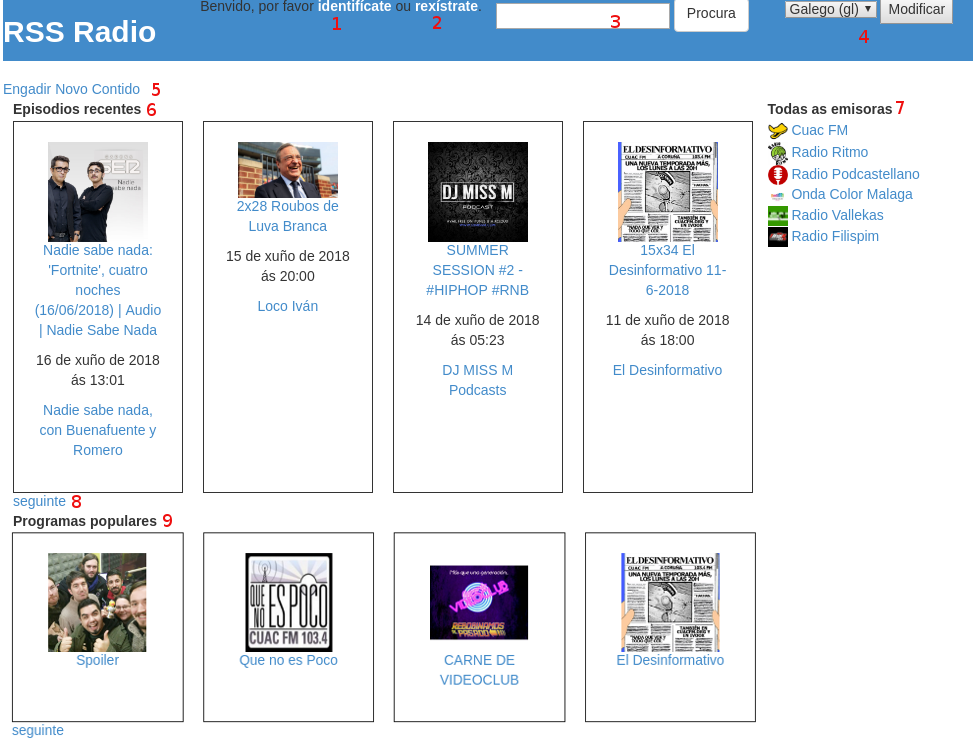
\includegraphics[scale=0.43,keepaspectratio=true]{./images/usermanual/um-index-anon.png}}
	\caption{Portada da web para usuario anónimo}
	\label{fig:um-index-anon}
\end{figure}

Na figura \ref{fig:um-index-anon} amósase o aspecto da portada da web para un usuario anónimo con números identificando as distintas áreas:

\begin{itemize}
	\item \textbf{1:} Enlace á páxina de login.
	\item \textbf{2:} Enlace á páxina de rexistro.
	\item \textbf{3:} Caixa de procura por texto.
	\item \textbf{4:} Selector de idioma.
	\item \textbf{5:} Enlace ao menú de creación de novo programa e emisora. Require identificación.
	\item \textbf{6:} Sección de episodios recentes. Amósanse os 4 últimos episodios engadidos ao sistema independentemente do seu programa. Para ver os 4 seguintes, pódese premer o botón marcado co \textbf{8}.
	\item \textbf{7:} Lista de emisoras presentes no sistema.
	\item \textbf{8:} Botón para cargar a seguinte páxina.
	\item \textbf{9:} Sección de programas ordenados por popularidade. Amósanse os 4 primeiros tamén con opción de cargar a seguinte páxina.  
\end{itemize}

\section{Usuarios}

\subsection{Crear}
Para crear un novo usuario, prémese un botón \textbf{2} da figura \ref{fig:um-index-anon}. Cargarase a páxina de rexistro de usuario. Basta con cubrir os campos como se amosa no exemplo da figura \ref{fig:um-signup}. Se non hai ningún erro, o usuario quedará autenticado e será redirixido á súa páxina de detalles (figura \ref{fig:um-userd1})



\subsection{Editar}
Para acceder ao menú de edición de usuario, prémese o botón de edición marcado co \textbf{10} na figura \ref{fig:um-userd1}. O menú de edición pódese ver na figura \ref{fig:um-edituser}. Nótese que o nome de usuario non é editable e que o cambio de password é un formulario aparte.

Se a edición se completa de forma correcta, vólvese á vista de detalles de usuario.

\begin{figure}[H]
	\centering
	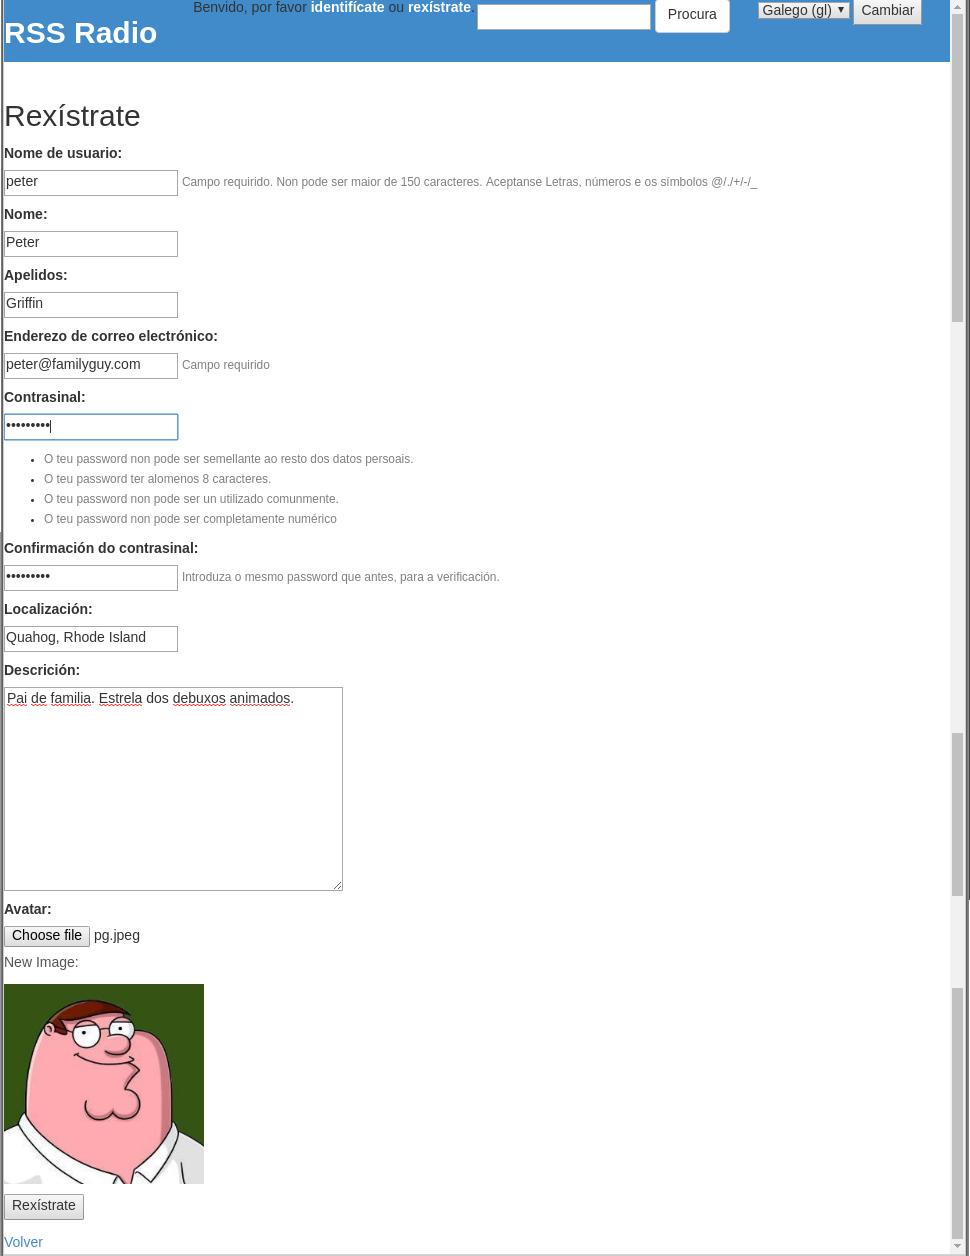
\includegraphics[scale=0.43,keepaspectratio=true]{./images/usermanual/um-signup.png}
	\caption{Rexistro de usuario.}
	\label{fig:um-signup}
\end{figure}


\begin{figure}[H]
	\centering
	\fbox{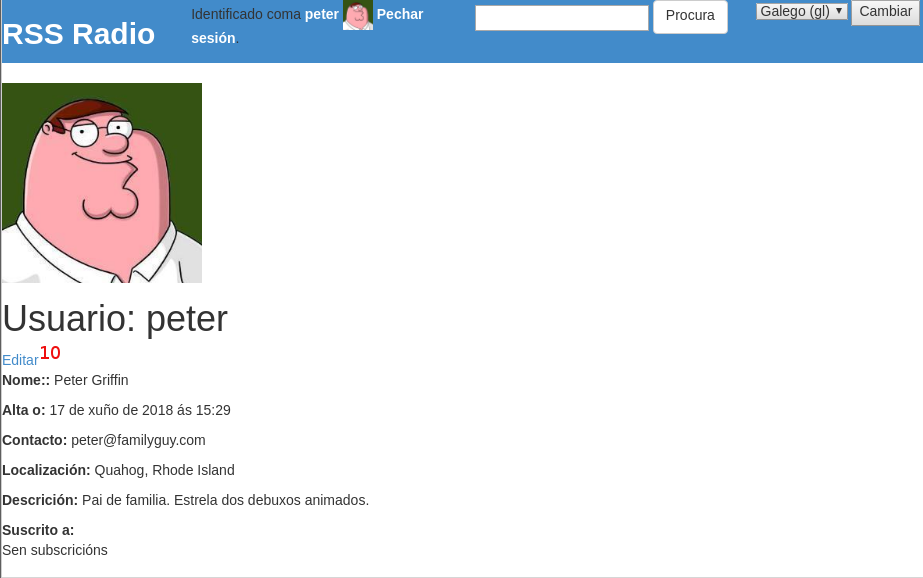
\includegraphics[scale=0.45,keepaspectratio=true]{./images/usermanual/um-userd1.png}}
	\caption{Detalles de usuario. Información do perfil.}
	\label{fig:um-userd1}
\end{figure}


\begin{figure}[H]
	\centering
	\fbox{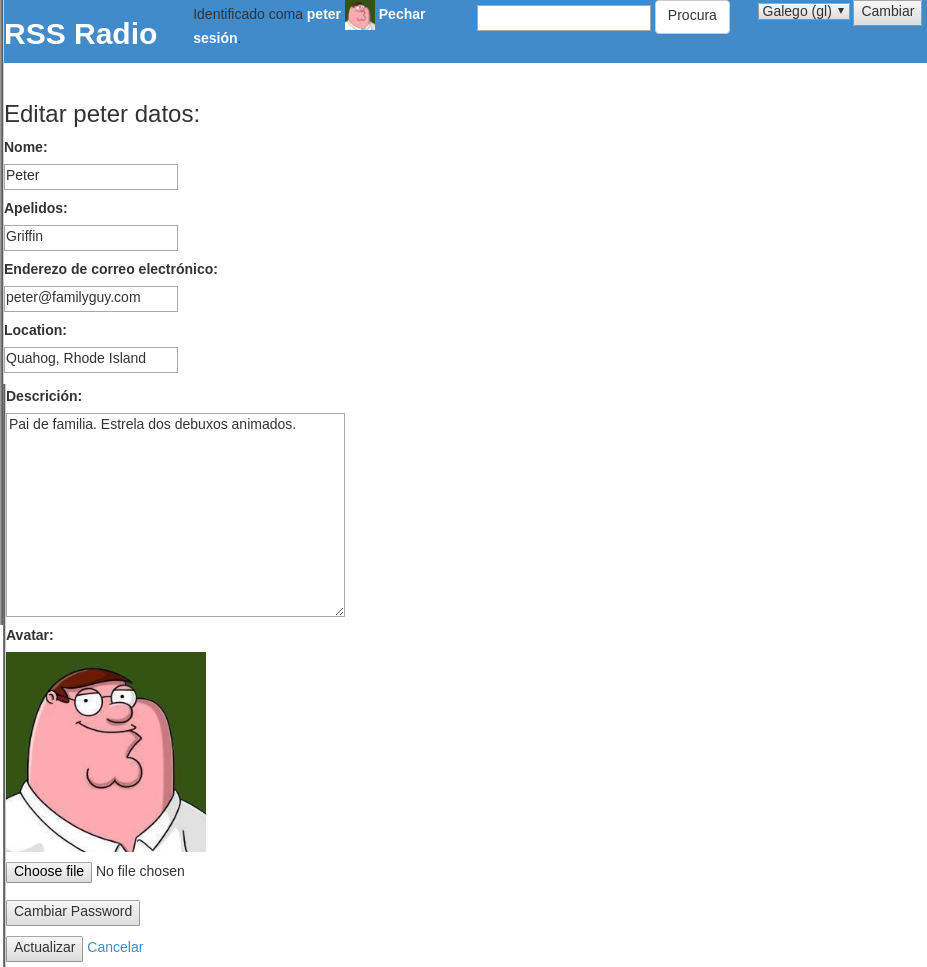
\includegraphics[scale=0.45,keepaspectratio=true]{./images/usermanual/um-edituser.png}}
	\caption{Editar usuario.}
	\label{fig:um-edituser}
\end{figure}


\section{Accións de ouvinte}

\subsection{Escoitar e seguir unha emisora}

Para realizar accións sobre unha emisora cómpre ir á súa páxina de detalles. As emisoras poden ser \say{seguidas} polos usuarios como forma de engadila a \say{favoritas}. A continuación explícanse os elementos da páxina de detalles de emisora marcados na figura \ref{fig:um-stationd1}.

\begin{itemize}
	\item \textbf{11:} Botón de seguimento.
	\item \textbf{12:} Reprodutor de emisión en directo.
	\item \textbf{13:} Lista dos últimos episodios publicados ordenada por data.
	\item \textbf{14:} Lista de programas emitidos pola emisora.
	\item \textbf{15:} Usuarios seguidores  da emisora.
\end{itemize}


\subsection{Subscribirse a un programa}

Para subscribirse ou cancelar unha subscrición previa, o usuario debe ir á páxina de detalles do programa en cuestión. A continuación explícanse os elementos da páxina de detalles de programa marcados na figura \ref{fig:um-programd1}.

\begin{itemize}
	\item \textbf{16:} Botón de subscrición.
	\item \textbf{17:} Enlace á páxina de resultados de busca polo tag \say{comedy}.
	\item \textbf{18:} Lista dos últimos episodios ordenada por data de publicación dos audios.
	\item \textbf{19:} Lista de emisoras nas que se emite o programa.
	\item \textbf{20:} Usuarios subscritos ao programa.
\end{itemize}

\subsection{Accións sobre os episodios}

Accedendo á vista de detalles de episodio pódese escoitar mediante streaming ou descargar o ficheiro de audio. Os episodios poden votarse e comentarse.  A continuación explícanse os elementos da páxina de detalles de episodio marcados na figura \ref{fig:um-episoded1}.

\begin{itemize}
	\item \textbf{21:} Botóns de voto positivo ou negativo. O usuario sempre pode desfacer ou cambiar o seu voto.
	\item \textbf{22:} Reprodutor do ficheiro de audio do episodio.
	\item \textbf{23:} Enlace á páxina de resultados de busca por tag (Neste exemplo, o episodio non ten tags de seu.)
	\item \textbf{24:} Sección de comentarios do episodio.
\end{itemize}

\begin{figure}[H]
	\centering
	\fbox{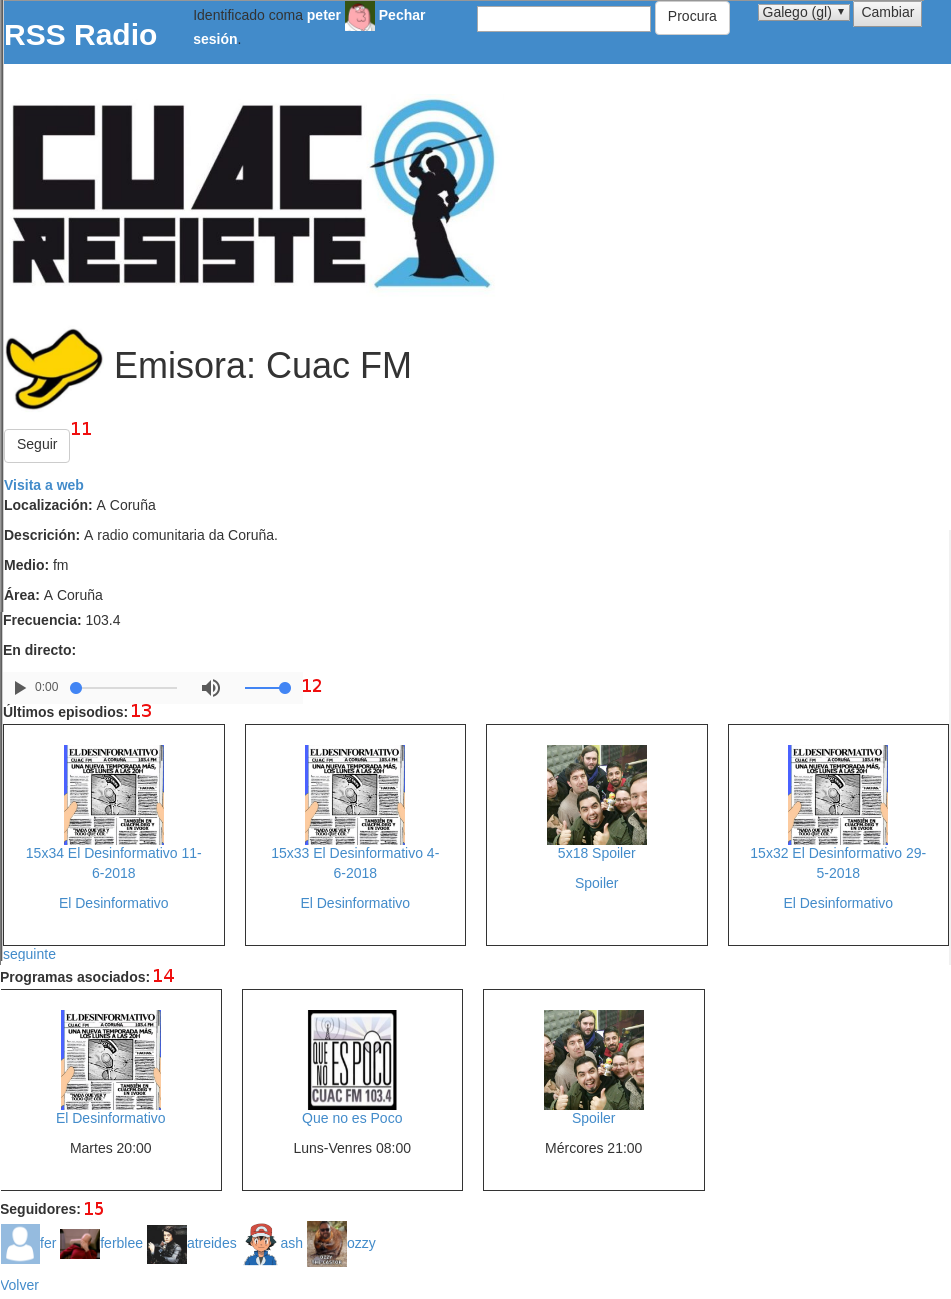
\includegraphics[scale=0.45,keepaspectratio=true]{./images/usermanual/um-stationd1.png}}
	\caption{Detalles de emisora.}
	\label{fig:um-stationd1}
\end{figure}

\begin{figure}[H]
	\centering
	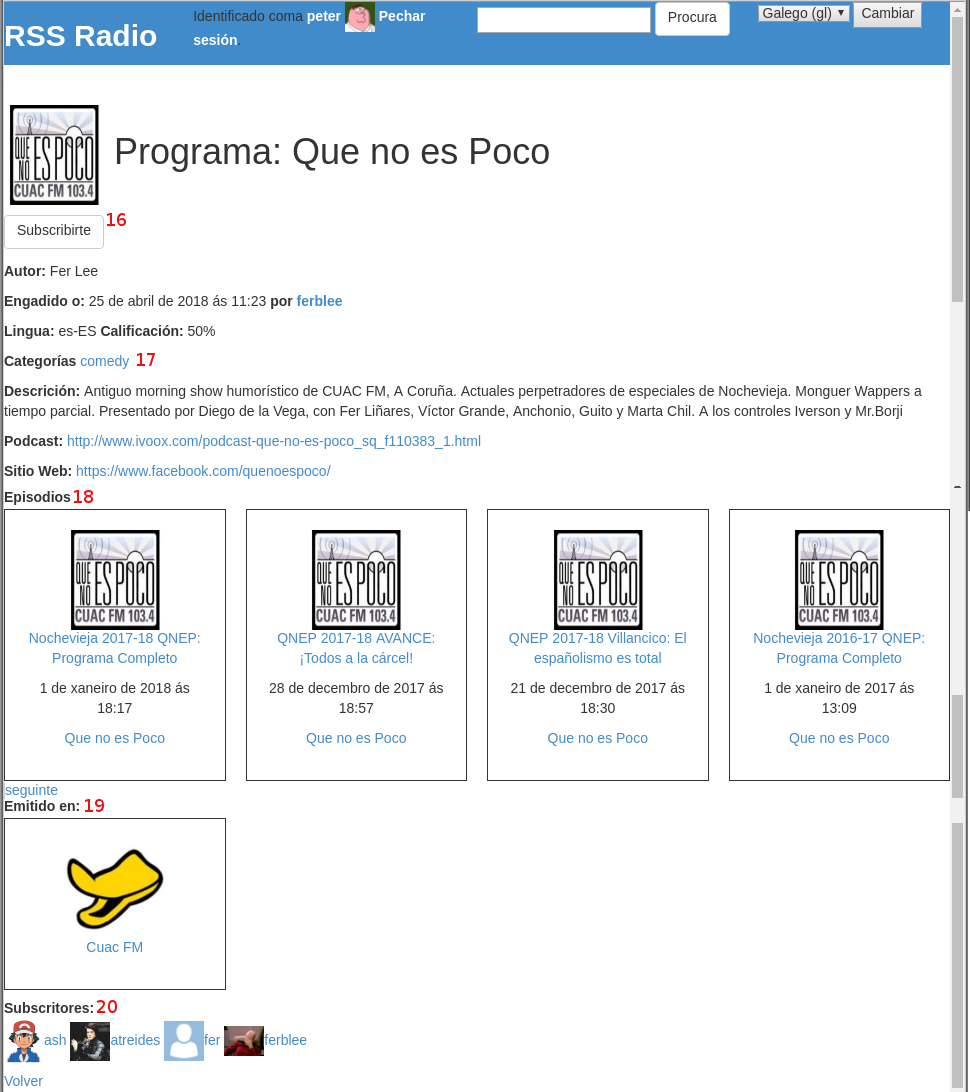
\includegraphics[scale=0.45,keepaspectratio=true]{./images/usermanual/um-programd1.png}
	\caption{Detalles de programa.}
	\label{fig:um-programd1}
\end{figure}


\begin{figure}[H]
	\centering
	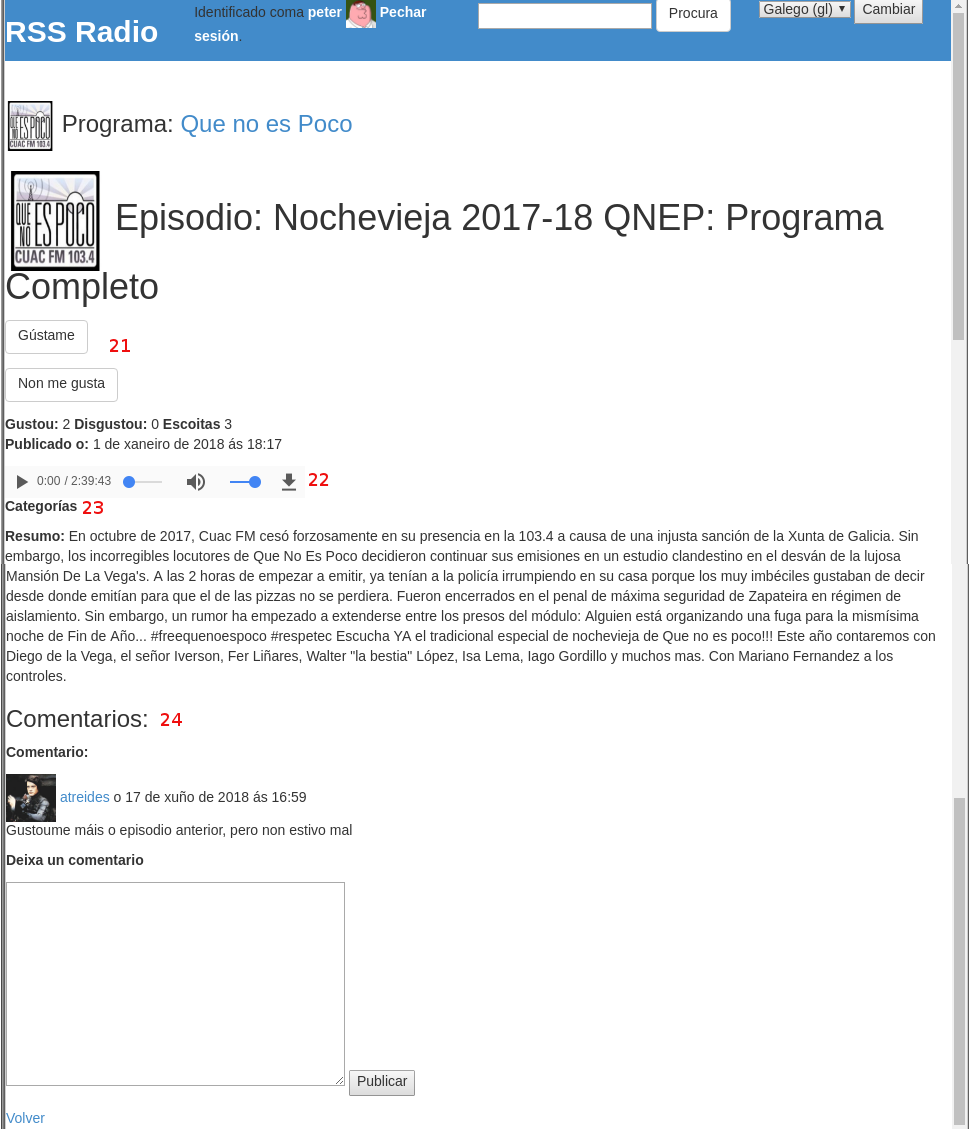
\includegraphics[scale=0.45,keepaspectratio=true]{./images/usermanual/um-episoded1.png}
	\caption{Detalles de episodio.}
	\label{fig:um-episoded1}
\end{figure}

\subsection{Contidos favoritos}

Nos exemplos anteriores, o usuario seguiu unha emisora e subscribiuse a un programa. Este contido está agora dispoñible de xeito máis fácil desde a portada e máis desde o seu perfil como se pode ver nas figuras \ref{fig:um-index-auth} e \ref{fig:um-userd2}.

\begin{figure}[H]
	\centering
	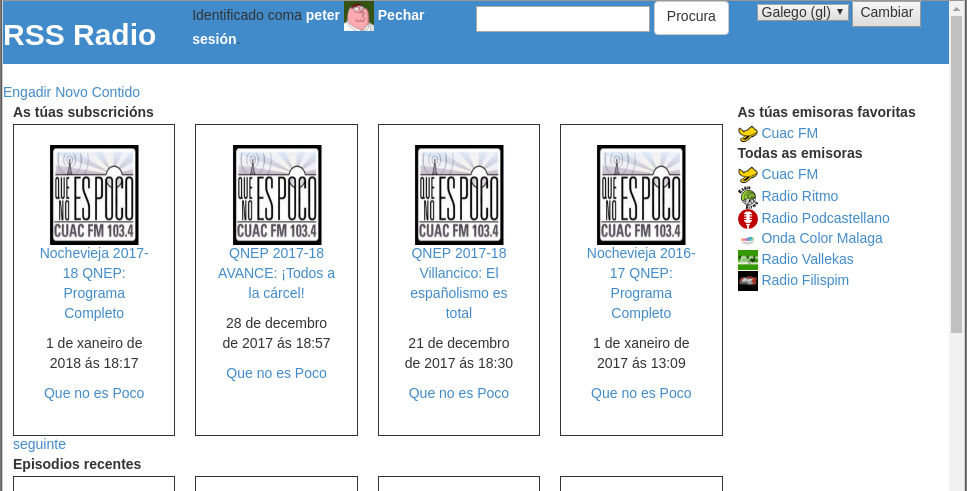
\includegraphics[scale=0.45,keepaspectratio=true]{./images/usermanual/um-index-auth.png}
	\caption{Contidos favoritos na portada.}
	\label{fig:um-index-auth}
\end{figure}


\begin{figure}[H]
	\centering
	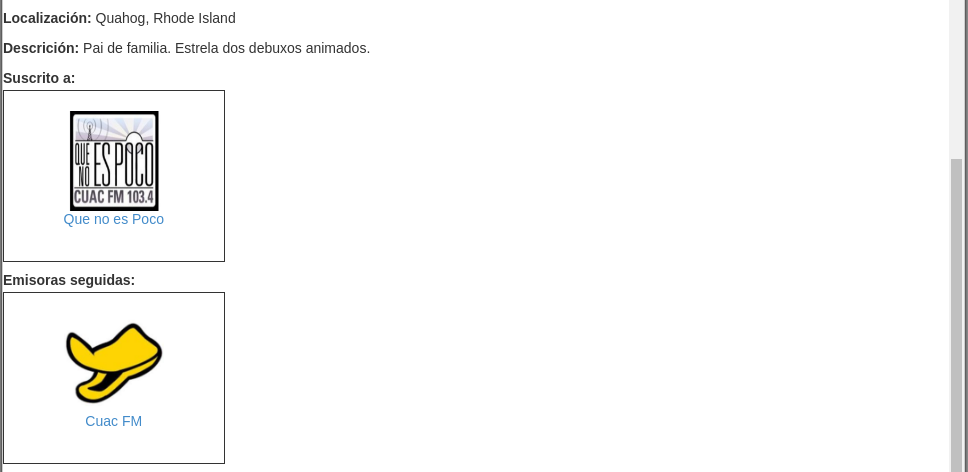
\includegraphics[scale=0.45,keepaspectratio=true]{./images/usermanual/um-userd2.png}
	\caption{Contidos favoritos na vista de perfil de usuario.}
	\label{fig:um-userd2}
\end{figure}


\section{Procura de contidos}

O sistema proporciona 2 formas de procura de contidos: Por texto, mediante a caixa marcada co \textbf{3} na figura \ref{fig:um-index-anon} , ou por tag, premendo nos enlaces correspondentes (Ver número \textbf{17} na figura \ref{fig:um-programd1}). Ambas levan á páxina de resultados de procura, onde se amosarán os episodios, programas, emisoras e usuarios que cumpran os criterios da busca.

Na figura \ref{fig:um-search} móstrase un exemplo de procura pola palabra \say{radio}.

\begin{figure}[H]
	\centering
	\fbox{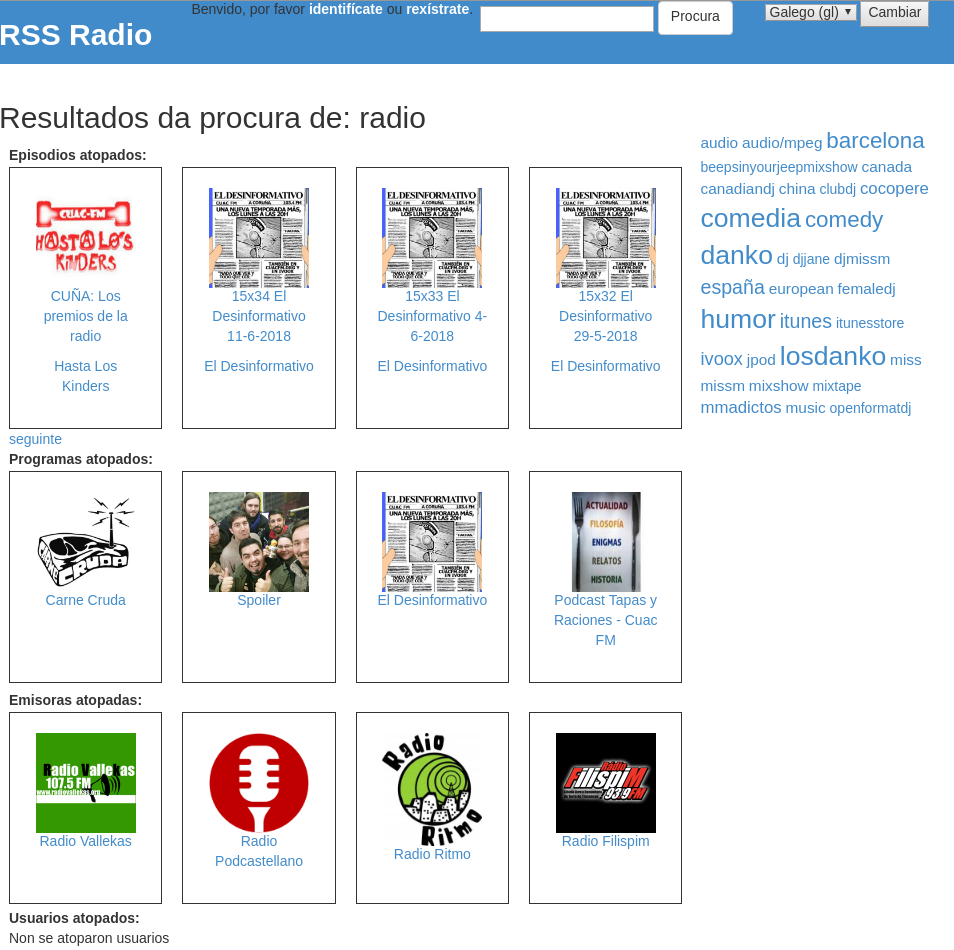
\includegraphics[scale=0.45,keepaspectratio=true]{./images/usermanual/um-search.png}}
	\caption{Páxina de resultados de procura. Exemplo de busca pola palabra radio.}
	\label{fig:um-search}
\end{figure}


\section{Accións de produtor de contidos}

\subsection{Crear unha emisora}

Para engadir unha emisora, o usuario ten que ir á vista de \say{engadir contido}, mediante o enlace marcado co \textbf{5} na figura 	\ref{fig:um-index-anon}. Unha vez alí, cóbrense os campos do formulario como se ve na figura \ref{fig:um-add-station}

Se os datos introducidos son correctos, rediríxese ao usuario á páxina de detalles da nova emisora (figura \ref{fig:um-stationd2}). O usuario creador da emisora ten permisos de \say{propietario} sobre a citada emisora.


\subsection{Xestionar unha emisora}

Se o usuario é propietario ou xestor dunha emisora, poderá ver o botón marcado coma \textbf{25} na figura \ref{fig:um-stationd2}. Este levaralle ao panel de xestión da emisora, no que se poden realizar as seguintes operacións:

\subsubsection{Editar perfil}

Vista amosada na figura \ref{fig:um-edstation1}. Desde ahí pódense editar os datos do perfil da emisora.


\subsubsection{Xestionar emisión}
\label{xe}

Vista amosada na figura \ref{fig:um-edstation2}. Desde aí pódense engadir programas á emisión e retiralos da mesma.

\begin{itemize}
	\item \textbf{26:} Selector de programa. Úsase para seleccionar o programa que se queira engadir á emisión.
	\item \textbf{27:} Caixa de texto para especificar o horario de emisión do programa a engadir.
	\item \textbf{28:} Área de programas xa emitidos. Ás filas seleccionadas aplicaráselles á acción definida en \textbf{29}.
	\item \textbf{29:} Botóns de acción. Determinan se os programas seleccionados son para borrar ou para actualizar os seus datos de emisión.
\end{itemize}

\begin{figure}[H]
	\centering
	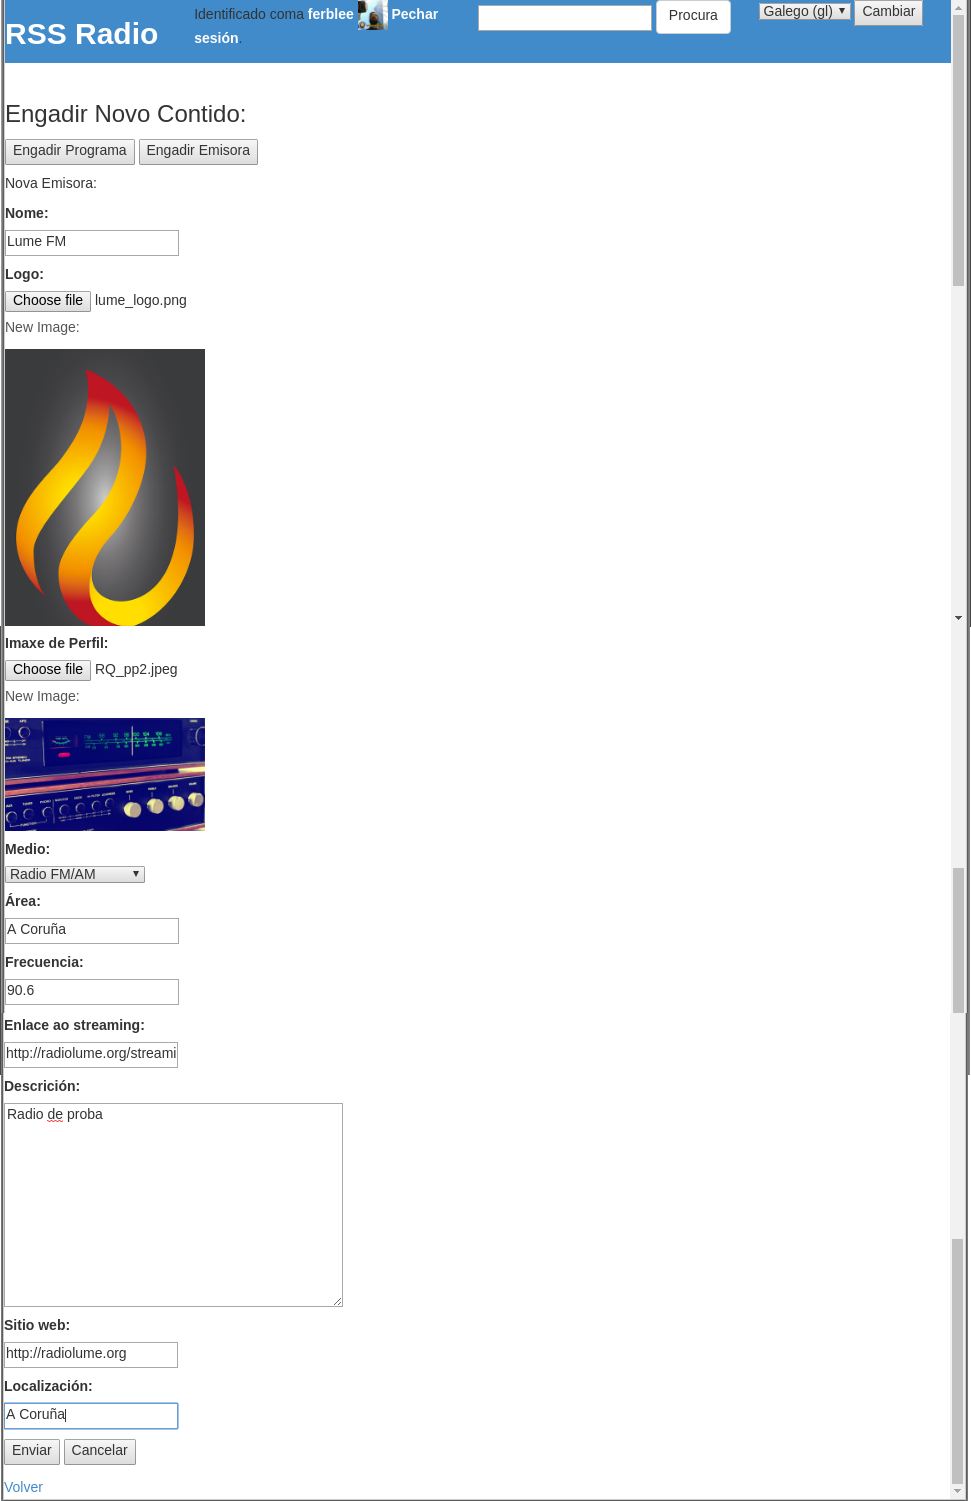
\includegraphics[scale=0.4,keepaspectratio=true]{./images/usermanual/um-add-station.png}
	\caption{Engadir emisora.}
	\label{fig:um-add-station}
\end{figure}

\break

\begin{figure}[H]
	\centering
	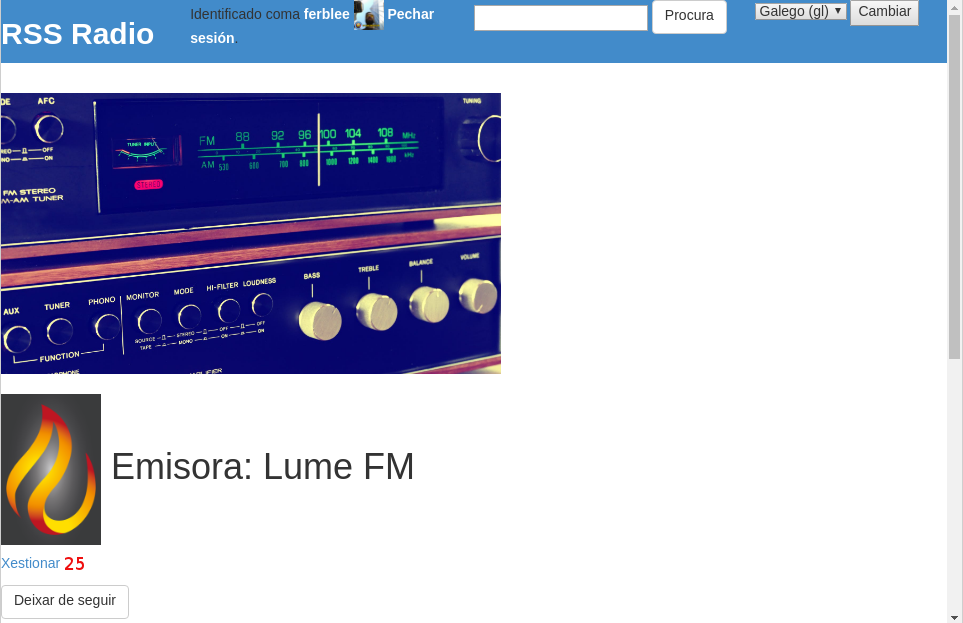
\includegraphics[scale=0.43,keepaspectratio=true]{./images/usermanual/um-stationd2.png}
	\caption{Vista de detalles de emisora: Nova emisora.}
	\label{fig:um-stationd2}
\end{figure}

\begin{figure}[H]
	\centering
	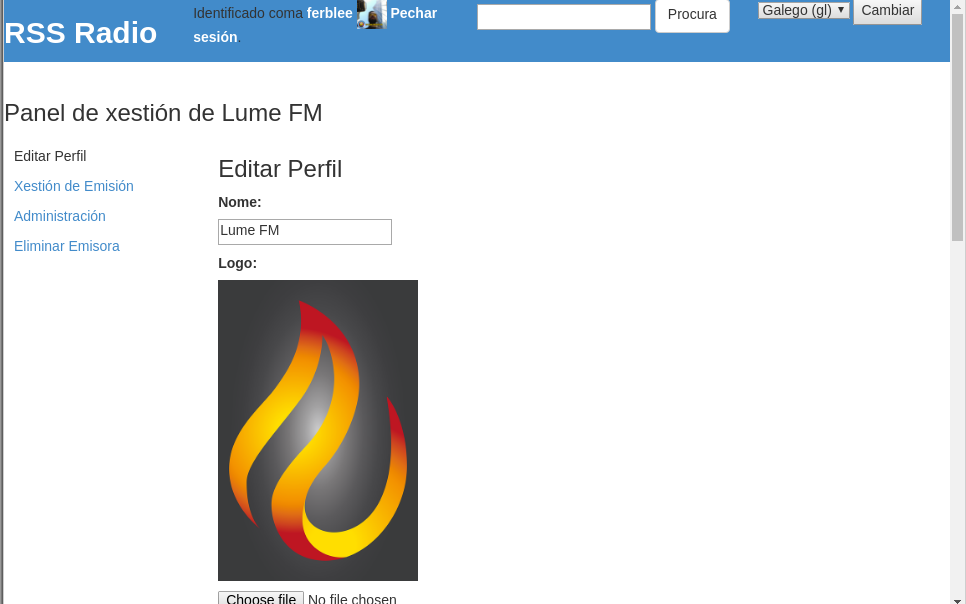
\includegraphics[scale=0.43,keepaspectratio=true]{./images/usermanual/um-edstation1.png}
	\caption{Panel de xestión de emisora: Editar perfil.}
	\label{fig:um-edstation1}
\end{figure}

\begin{figure}[H]
	\centering
	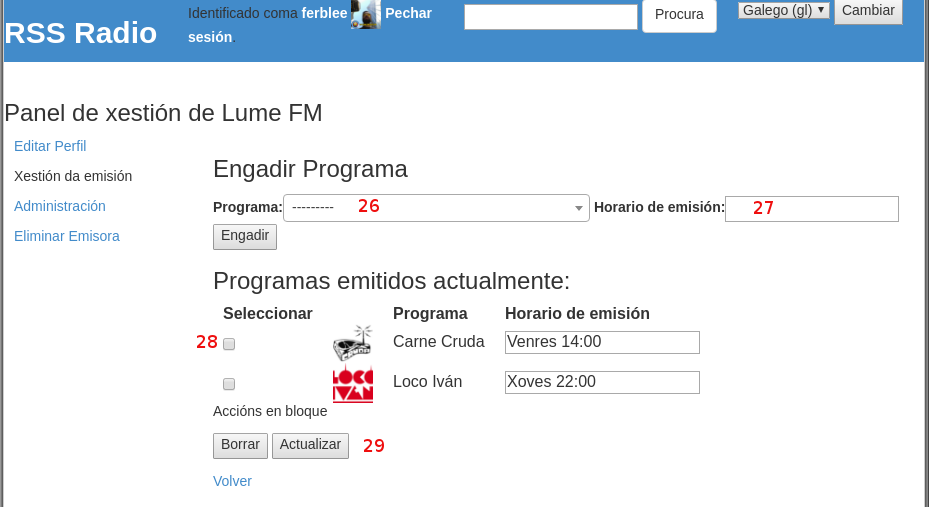
\includegraphics[scale=0.43,keepaspectratio=true]{./images/usermanual/um-edstation2.png}
	\caption{Panel de xestión de emisora: Xestionar emisión.}
	\label{fig:um-edstation2}
\end{figure}

\subsubsection{Xestionar administradores}
\label{xadmin}
Vista amosada na figura \ref{fig:um-edstation3}. Desde aí pódenselle conceder e revogar aos usuarios permisos sobre a emisora. Só os usuarios de nivel propietario poden acceder a esta vista. 

\textbf{Importante:} O propietario orixinal da emisora é o usuario que a crea. Este pode nomear outros propietarios pero, unha vez nomeados, non os poderá \say{degradar} xa que estarán ao seu mesmo nivel. Recoméndase prudencia á hora de conceder os permisos.

\begin{itemize}
	\item \textbf{30:} Selector de usuario. Úsase para seleccionar o usuario ao que se lle queiran dar permisos.
	\item \textbf{31:} Selector de permisos. Poden ser de administrador (limitados) ou de propietario (totais)
	\item \textbf{32:} Área de usuarios xa con permisos. Ás filas seleccionadas aplicaráselles á acción definida en \textbf{33}.
	\item \textbf{33:} Botóns de acción. Determinan se os usuarios seleccionados son para borrar ou para actualizar os seus permisos.
\end{itemize}


\subsubsection{Borrar emisora}

Vista amosada na figura \ref{fig:um-edstation4}. Desde aí pódese eliminar a emisora. So os propietarios teñen acceso a esta vista.

\begin{figure}[H]
	\centering
	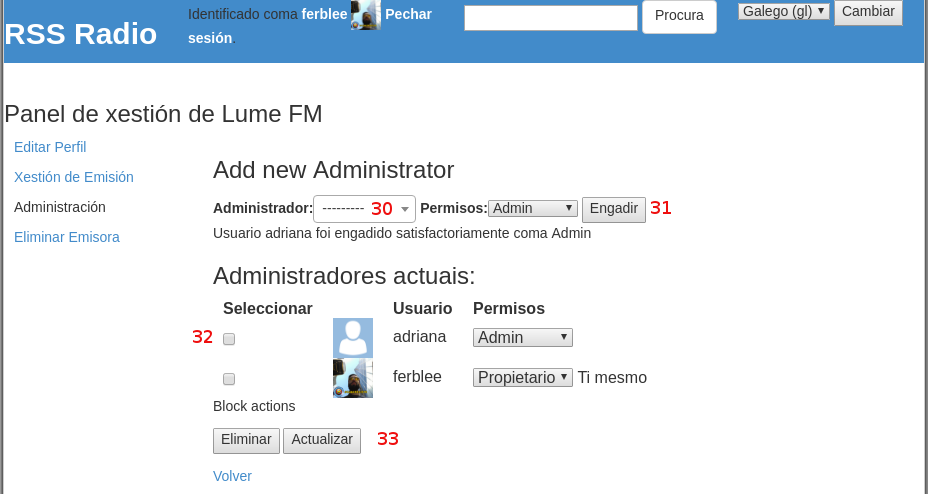
\includegraphics[scale=0.43,keepaspectratio=true]{./images/usermanual/um-edstation3.png}
	\caption{Panel de xestión de emisora: Xestionar administradores.}
	\label{fig:um-edstation3}
\end{figure}

\begin{figure}[H]
	\centering
	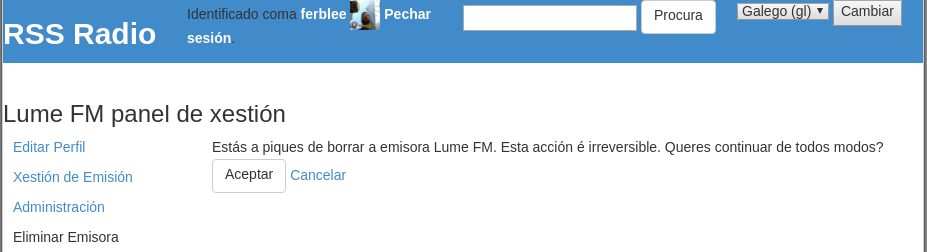
\includegraphics[scale=0.43,keepaspectratio=true]{./images/usermanual/um-edstation4.png}
	\caption{Panel de xestión de emisora: Borrar emisora.}
	\label{fig:um-edstation4}
\end{figure}


\subsection{Crear un programa}

Ao igual que a emisora, é necesario acceder ao menú de engadir contido a través do botón \textbf{5} na figura \ref{fig:um-index-anon} e cubrir o formulario que se ve na figura \ref{fig:um-add-program}.

Se os datos introducidos son correctos, rediríxese ao usuario á páxina de detalles da novo programa (figura \ref{fig:um-programd2}), onde tamén poderemos ver todos os seus episodios, creados automaticamente. O usuario creador do programa ten permisos de \say{propietario} sobre el e mailos seus episodios.

\begin{itemize}
	\item \textbf{34:} Opcións de compartición. As opcións son \textit{libre} e \textit{desactivada} segundo se desexe que as emisoras poidan emitir libremente o novo programa ou non.  
	\item \textbf{35:} Opcións de comentarios. As opcións son \textit{Permitir} e \textit{Deshabilitar} os comentarios nos episodios do novo programa.
\end{itemize}


\begin{figure}[H]
	\centering
	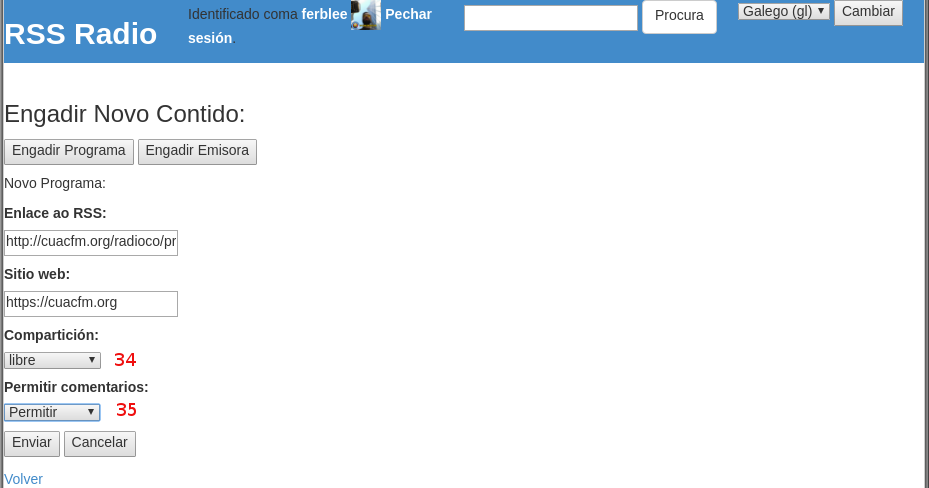
\includegraphics[scale=0.43,keepaspectratio=true]{./images/usermanual/um-add-program.png}
	\caption{Engadir programa.}
	\label{fig:um-add-program}
\end{figure}

\begin{figure}[H]
	\centering
	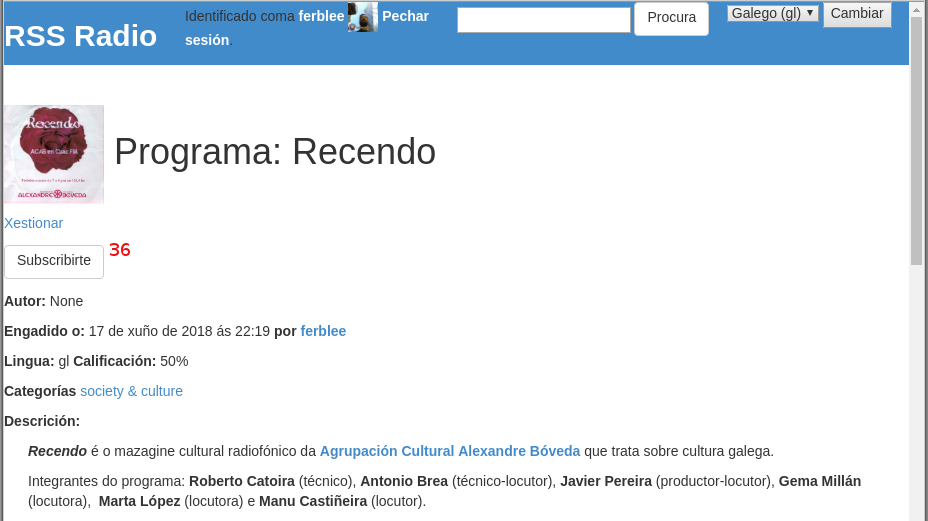
\includegraphics[scale=0.43,keepaspectratio=true]{./images/usermanual/um-programd2.png}
	\caption{Vista de detalles de program: Novo programa.}
	\label{fig:um-programd2}
\end{figure}


\subsection{Xestionar un programa}

Se o usuario é propietario ou xestor dun programa, poderá ver o botón marcado coma \textbf{36} na figura \ref{fig:um-programd2} que leva ao panel de xestión do programa. O sistema non ofrece ferramentas de xestión non edición dos episodios de xeito individual. As opcións definidas para o programa aplicaranse a todos os seus episodios sen excepcións.

As ferramentas que se utilizan neste panel funcionan do mesmo xeito que as do panel de xestión de emisora. Ante calquera dúbida, consultar as seccións \ref{xe} e \ref{xadmin}.

Neste panel pódense realizar as seguintes operacións:

\subsubsection{Editar perfil}

Esta vista é semellante á de editar o perfil da emisora, porén, podemos ver na \ref{fig:um-edprogram1} que as opcións son, aquí, moito máis limitadas debido a que a información é obtida dunha fonte externa (o ficheiro RSS) e non da entrada manual de datos por parte do usuario.

\begin{figure}[h]
	\centering
	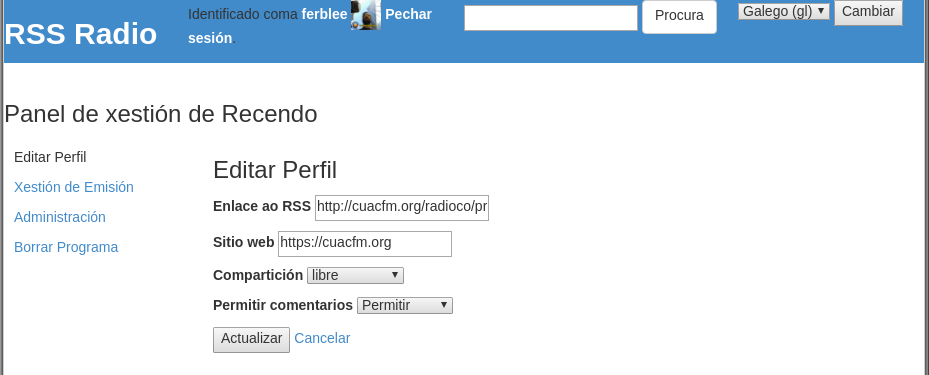
\includegraphics[scale=0.43,keepaspectratio=true]{./images/usermanual/um-edprogram1.png}
	\caption{Panel de xestión de programa: Editar perfil.}
	\label{fig:um-edprogram1}
\end{figure}

\subsubsection{Xestionar emisión}

Vista amosada na figura \ref{fig:um-edprogram2}. O sistema dá a oportunidade ao propietario do programa de cesar a emisión nunha emisora, pero, como é lóxico, non de modificar o seu horario de emisión nesa emisora. 

\begin{figure}[h]
	\centering
	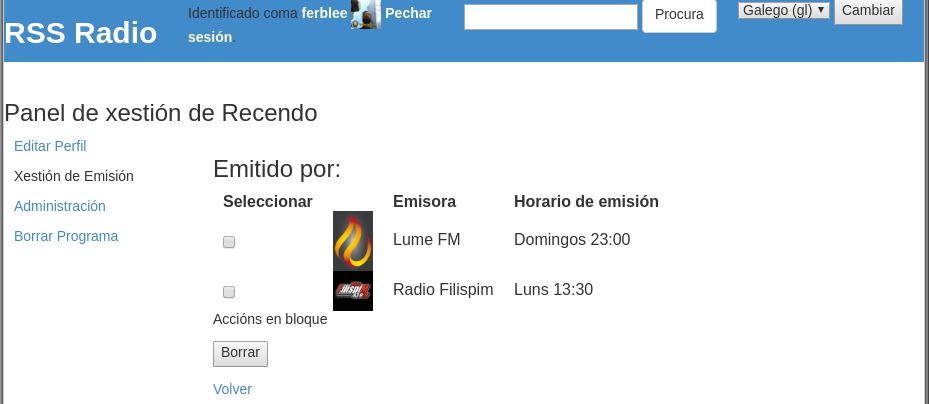
\includegraphics[scale=0.43,keepaspectratio=true]{./images/usermanual/um-edprogram2.png}
	\caption{Panel de xestión de programa: Xestionar emisión.}
	\label{fig:um-edprogram2}
\end{figure}

\subsubsection{Xestionar administradores}

Vista amosada na figura \ref{fig:um-edprogram3}. Desde aí pódenselle conceder e revogar aos usuarios permisos sobre a emisora. Só os usuarios de nivel propietario poden acceder a esta vista. 

\textbf{Importante:} O propietario orixinal do programa é o usuario que o crea. Este pode nomear outros propietarios pero, unha vez nomeados, non os poderá \say{degradar} xa que estarán ao seu mesmo nivel. Recoméndase prudencia á hora de conceder os permisos.

\begin{figure}[h]
	\centering
	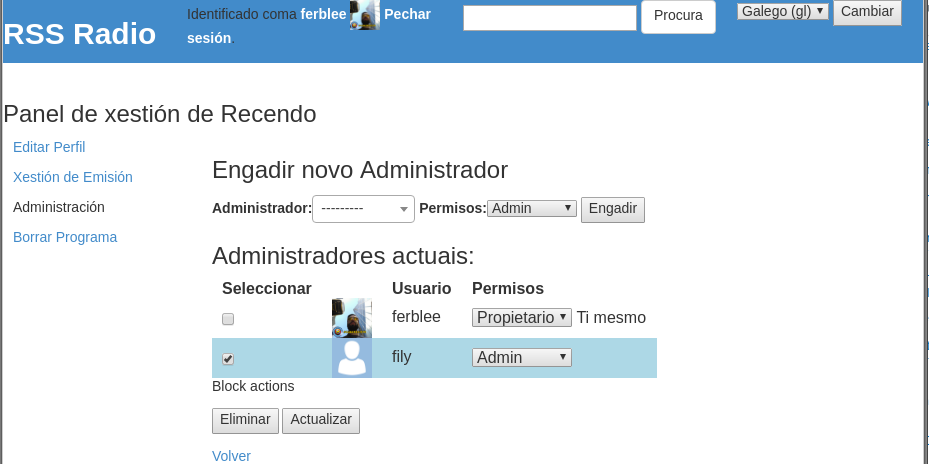
\includegraphics[scale=0.43,keepaspectratio=true]{./images/usermanual/um-edprogram3.png}
	\caption{Panel de xestión de programa: Xestionar administradores.}
	\label{fig:um-edprogram3}
\end{figure}


\subsubsection{Borrar programa}

Vista amosada na figura \ref{fig:um-edprogram4}. Desde aí pódese eliminar o programa. So os propietarios teñen acceso a esta vista.

\textbf{Importante:} O borrado dun programa implica a eliminación de todos os seus episodios así como das súas imaxes relacionadas. Os datos non serán recuperables.

\begin{figure}[h]
	\centering
	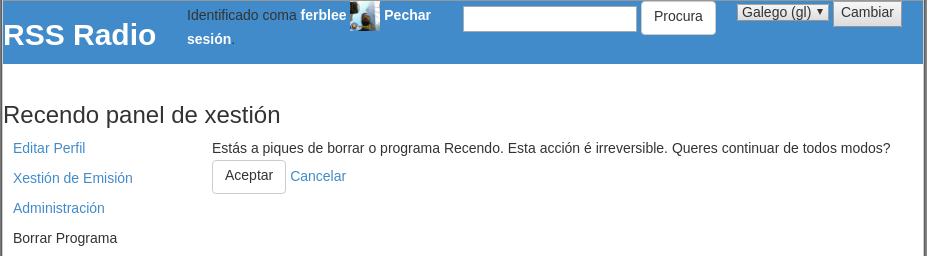
\includegraphics[scale=0.43,keepaspectratio=true]{./images/usermanual/um-edprogram4.png}
	\caption{Panel de xestión de programa: Borrar programa.}
	\label{fig:um-edprogram4}
\end{figure}
  % Glossary
  %\printglossary[title=Glosario,toctitle=Glosario]
  %\printglossary[type=\acronymtype,title=Acrónimos,toctitle=Acrónimos]
  % Bibliography
  %\nocite{*}    % incluir referencias no citadas.
  %\bibliographystyle{plainnat}
  \bibliographystyle{unsrtnat}
  %\bibliographystyle{ksfh_nat}
  %\bibliographystyle{dcu}  % Books and web
  \bibliography{pfc}

  
\end{document}

